\documentclass{article}
\title{Multivariable Calculus Concise Review} % title - chapter number
\author{John Yang}
\usepackage{amsmath}
\usepackage{amssymb}
\usepackage[margin=0.775in, letterpaper]{geometry}
\usepackage{outlines}
\usepackage{multicol}
\setcounter{section}{+10} % chapter number minus 1
\usepackage{mathtools}
\usepackage{physics}
\usepackage{esint}
\usepackage{stackrel}
\DeclarePairedDelimiter\set\{\}

\usepackage{graphicx}
\graphicspath{ {./} }

\usepackage{hyperref}
\hypersetup{
	colorlinks=true,
	linkcolor=blue,
	filecolor=magenta,      
	urlcolor=cyan,
}
\usepackage{tocloft}
\renewcommand\cftsecfont{\normalfont}
\renewcommand\cftsecpagefont{\normalfont}
\renewcommand{\cftsecleader}{\cftdotfill{\cftsecdotsep}}
\renewcommand\cftsecdotsep{\cftdot}
\renewcommand\cftsubsecdotsep{\cftdot}

\usepackage{fancyhdr}

\pagestyle{fancy}
\fancyhf{}
\rhead{John Yang}
\lhead{MC Concise Review}
\rfoot{Pg. \thepage}

\begin{document}
    \maketitle
    \tableofcontents\newpage
    
    \section{Parametric Equations and Polar Coordinates} % chapter title
    
    \subsection{Curves Defined by Parametric Equations} % section topic
    \begin{outline}
        \1 Parameter - 3rd variable that $x$ and $y$ are both a function of: \[x=f(t)\text{ and }y=g(t)\]
        \1 Points along the curve \((x,y)=(f(t),g(t))\)
        \1 Graphing calculators can be used to produce parametric curves that you wouldn't be able to make by hand. 
        \1 Parametric equations for a cycloid: \[x=r(\theta-\sin\theta) \qquad y=r(1-\cos\theta) \qquad \theta\in\mathbb{R}\]
    \end{outline}
    \subsection{Calculus with Parametric Curves}
    \begin{outline}
        \1 First derivative of a parametric equation: \[\dfrac{dy}{dx}=\dfrac{\dfrac{dy}{dt}}{\dfrac{dx}{dt}}\qquad\qquad\text{if}\quad\dfrac{dx}{dt}\neq0\]
        \1 Second derivative of a parametric equation: \[\dfrac{d^2y}{dx^2}=\dfrac{d}{dx}\left(\dfrac{dy}{dx}\right)=\dfrac{\dfrac{d}{dt}\left(\dfrac{dy}{dx}\right)}{\dfrac{dx}{dt}}\neq\dfrac{\dfrac{d^2}{dt^2}}{\dfrac{d^2x}{dt^2}}\]
        \1 Arc length of a curve: \[L=\int^b_a\sqrt{1+\left(\dfrac{dy}{dx}\right)^2}dx\]
        \1 Arc length of a parametric curve: \[L=\int^\beta_\alpha\sqrt{\left(\dfrac{dx}{dt}\right)^2+\left(\dfrac{dy}{dt}\right)^2}dt\]
        \1 Surface area of a rotated parametric curve about the $x$ axis: \[S=\int^\beta_\alpha2\pi y\sqrt{\left(\dfrac{dx}{dt}\right)^2+\left(\dfrac{dy}{dt}\right)^2}dt\]

    \end{outline}
    \subsection{Polar Coordinates}
    \begin{outline}
        \1 polar coordinates - \((r,\theta)\)
        \1 Theta is always ccw 
        \1 Polar coordinates: \[x=r\cos\theta\qquad\qquad y=r\sin\theta\]\[r^2=x^2+y^2\qquad\qquad\tan\theta=\dfrac{y}{x}\]
        \1 Derivative of a polar curve: \[\dfrac{dy}{dx}=\dfrac{\dfrac{dy}{d\theta}}{\dfrac{dx}{d\theta}}=\dfrac{\dfrac{dr}{d\theta}\sin\theta+r\cos\theta}{\dfrac{dr}{d\theta}\cos\theta-r\sin\theta}\]
    \end{outline}
    \subsection{Areas and Lengths in Polar Coordinates}
    \begin{outline}
        \1 Area of a sector of a circle: \(A=\frac{1}{2}r^2\theta\)
        \1 Polar area: \[A=\int^b_a\frac{1}{2}[f(\theta)]^2d\theta=\int^b_a\frac{1}{2}r^2d\theta\]
        \1 Polar arc length: \[L=\int^b_a\sqrt{r^2+\left(\dfrac{dr}{d\theta}\right)^2}d\theta\]
    \end{outline}
    \subsection{Conic Sections}
    \begin{outline}
        \1 Vertical parabola with focus \((0,p)\) and directrix \(y=-p\): \[x^2=4py\]
        \1 Horizontal parabola with focus \((p,0)\) and directrix \(x=-p\): \[y^2=4px\]
        \1 General form of an ellipse: \[\dfrac{x^2}{a^2}+\dfrac{y^2}{b^2}=1\]
        \1 Horizontal ellipse with foci \((\pm c,0)\), verticies \((\pm a,0)\), where \(c^2=a^2-b^2\) \[\dfrac{x^2}{a^2}+\dfrac{y^2}{b^2}=1\qquad a\geq b>0\]
        \1 Vertical ellipse with foci \((0,\pm c)\), verticies \((0,\pm a)\), where \(c^2=a^2-b^2\) \[\dfrac{x^2}{b^2}+\dfrac{y^2}{a^2}=1\qquad a\geq b>0\]
        \1 General form of a hyperbola: \[\dfrac{x^2}{a^2}-\dfrac{y^2}{b^2}=1\]
        \1 Hyperbola with horizontal transverse axis, with foci \((\pm c,0)\), verticies \((\pm a,0)\), asymptotes \(y=\pm\dfrac{b}{a}x\), where \(c^2=a^2+b^2\): \[\dfrac{x^2}{a^2}-\dfrac{y^2}{b^2}=1\]
        \1 Hyperbola with vertical transverse axis, foci \((0,\pm c)\), verticies \((0,\pm a)\), asymptotes \(y=\pm\dfrac{a}{b}x\), where \(c^2=a^2+b^2\): \[\dfrac{y^2}{a^2}-\dfrac{x^2}{b^2}=1\]

    \end{outline}
    \subsection{Conic Sections in Polar Coordinates}
    \begin{outline}
        \1 Let $F$ be a fixed point (called the focus) and $l$ be a fixed line (called the directrix) in a plane. Let $e$ be a fixed positive number (called the eccentricity). The set of all points $P$ in the plane such that \[\dfrac{|PF|}{|Pl|}=e\] is a conic section. (That is, the ratio of the distance from $F$ to the distance from $l$ is the constant $e$). The conic is: 
            \2 (a) an ellipse if \(e<1\)
            \2 a parabola if \(e=1\)
            \2 a hyperbola if \(e>1\)
        \1 A polar equation of the form \[r=\dfrac{ed}{1\pm e\cos\theta}\qquad\text{or}\qquad r=\dfrac{ed}{1\pm e\sin\theta}\] represents a conic section with eccentricity $e$. The conic is an ellipse if \(e<1\), parabola if \(e=1\), or a hyperbola if \(e>1\)
            \2 $d$ is the distance from focus to directrix
        \1 \(e=\dfrac{c}{a}\qquad\text{where}\qquad c^2=a^2+b^2\)
        \1 Kepler's laws: 
            \2 1 - A planet revolves around the sun in an elliptical orbit with the sun at one focus. 
            \2 2 - The line joining the sun to a planet sweeps out equal areas in equal times. 
            \2 3 - The square of the period of revolution of a planet is proportional to the cube of the length of the major axis of its orbit. 
        \1 The polar equation of an ellpise with focus at the origin, semimajor axis $a$, eccentricity $e$, and directirx \(x=d\) can be written in the form: \[r=\dfrac{a(1-e^2)}{1+e\cos\theta}\]
        \1 The perihelion distance from a planet to the sun is \(a(1-e)\) and the aphelion distance is \(a(1+e)\)
    \end{outline}
    
    \section{Infinite Sequences and Series} % chapter title
    
    \subsection{Sequences} % section topic
    \begin{outline}
        \1 sequence - a list of numbers written in a definite order: \[a_1, a_2, a_3, a_4, \cdots, a_n, \cdots \]
        \1 $a_1$ - first term; $a_2$ - second term; $a_n$ - nth term 
        \1 For infinite series, every term $a_n$ has a successor $a_{n+1}$
        \1 Notation - the sequence \(\{a_1, a_2, a_3, \cdots\}\) can also be written as \[\{a_n\}\text{ or }\{a_n\}^\infty_{n=1}\] 
        \1 Limits of sequences: \[\lim_{n\to\infty}a_n=L\]
            \2 This means: as $n$ becomes very large, the terms of the sequence $\{a_n\}$ approach $L$. 
        \1 can also be written as \[a_n\to L \text{ as } n\to\infty\]
        \1 If the limit at infinity exists, the sequence is convergent/converges. Otherwise, it is divergent/diverges. 
        \1 A more precise definition of the limit of a sequence: \[\lim_{n\to\infty}a_n=L\] if for every \(\varepsilon>0\) there is a corresponding integer $N$ such that \[\text{if }n>N\text{ then }|a_n-L|<\varepsilon\]
        \1 If \(\lim_{x\to\infty}f(x)=L\) and \(f(n)=a_n\) when $n$ is an integer, then \(\lim_{n\to\infty}a_n=L\). 
        \1 \[\lim_{n\to\infty}\dfrac{1}{n^r}=0\text{    if }r>0\]
        \1 \(\lim_{n\to\infty}a_n=\infty\) means that for every positive number M there is an integer $N$ such that \[\text{if }n>N\text{ then }a_n>M\]
    \end{outline}
    \begin{outline}
        \1 Limit laws for sequences: If \(\{a_n\}\text{ and }\{b_n\}\) are convergent sequences and $c$ is a constant, then: \[\lim_{n\to\infty}(a_n+b_n)=\lim_{n\to\infty}a_n+\lim_{n\to\infty}b_n\]\[\lim_{n\to\infty}(a_n-b_n)=\lim_{n\to\infty}a_n-\lim_{n\to\infty}b_n\]\[\lim_{n\to\infty}ca_n=c\lim_{n\to\infty}a_n\text{    }\lim_{n\to\infty}c=c\]\[\lim_{n\to\infty}(a_nb_n)=\lim_{n\to\infty}a_n\cdot\lim_{n\to\infty}b_n\]\[\lim_{n\to\infty}\dfrac{a_n}{b_n}=\dfrac{\lim_{n\to\infty}a_n}{\lim_{n\to\infty}b_n}\text{ if }\lim_{n\to\infty}b_n\neq0\]\[\lim_{n\to\infty}a_n^p=\left[\lim_{n\to\infty}a_n\right]^p\text{ if }p>0\text{ and }a_n>0\]
        \1 Squeeze Theorem can be adapted for sequences: \[\text{If }a_n\leq b_n\leq c_n\text{ for }n\geq n_0\text{ and }\lim_{n\to\infty}a_n=\lim_{n\to\infty}c_n=L\text{, then }\lim_{n\to\infty}b_n=L\]
        \1 \(\text{If }\lim_{n\to\infty}|a_n|=0\text{, then }\lim_{n\to\infty}a_n=0\)
    \end{outline}
        \begin{outline}
        \1 If \(\lim_{n\to\infty}a_n=L\) and the function f is continuous at $L$, then \[\lim_{n\to\infty}f(a_n)=f(L)\]
        \1 \[a_n=\dfrac{n!}{n^n}=\dfrac{1\cdot2\cdot3\cdot\cdots\cdot n}{n\cdot n\cdot n\cdot\cdots\cdot n}\] (ex. 10)
        \1 The sequence \(\{r^n\}\) is convergent if \(-1<r\leq 1\) and divergent for all other values of $r$. \[\lim_{n\to\infty}r^n=\begin{cases} 0 & \mbox{if } -1<r<1 \\ 1 & \mbox{if }r=1 \end{cases}\]
        \1 A sequence \(\{a_n\}\) is called \textbf{increasing} if \(a_n<a_{n+1}\) for all \(n\geq 1\), that is, \(a_1<a_2<a_3<\cdots\). It is called \textbf{decreasing} if \(a_n>a_{n+1}\) for all \(n\geq 1\). A sequence is \textbf{monotonic} if it is either increasing or decreasing. 
        \1 A sequence \(\{a_n\}\) is \textbf{bounded above} if there is a number $M$ such that \[a_n\leq M\mbox{    for all }n\geq 1\] It is bounded below if there is a number $m$ such that \[m\leq a_n\text{    for all }n\geq 1\] If it is bounded above and below, then \(\{a_n\}\) is a \textbf{bounded sequence}
        \1 Monotonic Sequence Theorem: Every bounded, monotonic sequence is convergent. 
        \1 Proof of the above: Suppose \(\{a_n\}\) is an increasing sequence. Since \(\{a_n\}\) is bounded, the set \(S=\{a_n|n\geq 1\}\) has an upper bound. By the Completeness Axiom it has a least upper bound $L$. Given \(\varepsilon>0\), \(L-\varepsilon\) is \textit{not} an upper bound for $S$ (since $L$ is the \textit{least} upper bound). Therefore \[a_N>L-\varepsilon\] For some integer $N$. But the sequence is increasing so \(a_n\geq a_N\) for every \(n>N\). Thus if \(n>N\), we have \[a_n>L-\varepsilon\] so \[0\leq L-a_n<\varepsilon\] since \(a_n\leq L\). Thus, \[|L-a_n|<\varepsilon\text{     whenever }n>N \] so \(\lim_{n\to\infty}a_n=L\). A similar proof can be applied if \(\{a_n\}\) is decreasing. 
    \end{outline}
    \subsection{Series}
    \begin{outline}
        \1 infinite series/series can be written as: \[a_1+a_2+a_3+\cdots+a_n+\cdots\]
        \1 Partial sums: \[s_n=a_1+a_2+a_3+\cdots+a_n=\sum^n_{i=1}a_i\] e.g. \[s_1=a_1\]\[s_2=a_1+a_2\]\[s_3=a_1+a_2+a_3\]\[s_4=a_1+a_2+a_3+a_4\]
        \1 given a series \(\sum^\infty_{n=1}a_n=a_1+a_2+a_3+\cdots\), its $n$th partial sum is denoted as above.
            \2 If the sequence \(\{s_n\}\) is convergent and \(\lim_{n\to\infty}s_n=s\) exists as a real number, then the series \(\sum a_n\) is called convergent and we write \[a_1+a_2+\cdots+a_n+\cdots=s\mbox{ or }\sum^\infty_{n=1}a_n=s\]
            \2 The number $s$ is called the sum of the series. If the sequence \(\{s_n\}\) is divergent, then the series is divergent. 
        \end{outline}
        \begin{outline}
            \1 Geometric series: \[a+ar+ar^2+ar^3+\cdots+ar^{n-1}+\cdots=\sum^\infty_{n=1}ar^{n-1}\mbox{ where }a\neq0\]
        \end{outline}
            \begin{outline}
        \1 sum of a geometric series \[s_n=\dfrac{a\left(1-r^n\right)}{1-r}\]
        \1 The geometric series \[\sum^\infty_{n=1}ar^{n-1}=a+ar+ar^2+\cdots\] is convergent if \(|r|<1\) and its sum is \[\sum^\infty_{n=1}ar^{n-1}=\dfrac{a}{1-r}\mbox{ where }|r|<1\] If \(|r|\geq1\), the geometric series is divergent. 
        \1 \[\sum^\infty_{n=0}x^n=\dfrac{1}{1-x}\]
        \1 If the series \(\sum^\infty_{n=1}a_n\) is convergent, then \(\lim_{n\to\infty}a_n=0\)
            \2 Note: The converse of this theorem is not always true!
        \1 Nth term test: If \(\lim_{n\to\infty}a_n\) does not exist or if \(\lim_{n\to\infty}a_n\neq0\), then the series \(\sum_{n=1}^\infty a_n\) is divergent. 
        \1 If \(\Sigma a_n\) and \(\Sigma b_n\) are convergent series, then so are the series \(\Sigma ca_n\) (where $c$ is a constant), \(\Sigma\left(a_n+b_n\right)\), and \(\Sigma\left(a_n-b_n\right)\), and \[\sum^\infty_{n=1}ca_n=c\sum^\infty_{n=1}a_n\]\[\sum^\infty_{n=1}\left(a_n+b_n\right)=\sum^\infty_{n=1}a_n+\sum^\infty_{n=1}b_n\]\[\sum^\infty_{n=1}\left(a_n-b_n\right)=\sum^\infty_{n=1}a_n-\sum^\infty_{n=1}b_n\]

    \end{outline}
    \subsection{The Integral Test and Estimates of Sums}
    \begin{outline}
        \1 The Integral Test: Suppose $f$ is a continuous, positive, decreasing function on \([1,\infty)\) and let \(a_n=f(n)\). Then the series \(\sum^\infty_{n=1}a_n\) is convergent IFF the proper integral \(\int^\infty_1f(x)dx\) is convergent. 
            \2 CONDITIONS: continuous, positive, decreasing function 
            \2 The integral from $1$ to $\infty$ of the function must be convergent for the series to be convergent. 
        \1 P-series test: The $p$-series \(\sum^\infty_{n=1}\dfrac{1}{n^p}\) is convergent if \(p>1\) and divergent if \(p\leq1\)
        \1 Remainder Estimate for the Integral Test: Suppose \(f(k)=a_k\), where $f$ is a continuous, positive, decreasing function for \(x\geq n\) and \(\Sigma a_n\) is convergent. If \(R_n=s-s_n\), then \[\int^\infty_{n+1}f(x)dx\leq R_n\leq\int^\infty_n f(x)dx\]
        \1 \[s_n+\int^\infty_{n+1}f(x)dx\leq s\leq s_n+\int^\infty_nf(x)dx\]
        \1 \[a_2+a_3+\cdots+a_n\leq\int^n_1f(x)dx\]
        \1 \[\int^n_1f(x)dx\leq a_1+a_2+\cdots+a_{n-1}\]
            \2 Both of the above two equations depend on the fact that $f$ is decreasing and positive. 
    \end{outline}
    \subsection{The Comparison Tests}
    \begin{outline}
        \1 The comparison test: Suppose that \(\Sigma a_n\) and \(\Sigma b_n\) are series with positive terms. 
            \2 If \(\Sigma b_n\) is convergent and \(a_n\leq b_n\) for all $n$, then \(\Sigma a_n\) is also convergent. 
            \2 If \(\Sigma b_n\) is divergent and \(a_n\geq b_n\) for all $n$, then \(\Sigma a_n\) is also divergent. 
        \1 The Limit comparison test: Suppose that \(\Sigma a_n\) and \(\Sigma b_n\) are series with positive terms. If \[\lim_{n\to\infty}\dfrac{a_n}{b_n}=c\] where $c$ is a finite number and \(c>0\), then either both series converge or both series diverge. 

    \end{outline}
    \subsection{Alternating Series}
    \begin{outline}
        \1 The alternating series test: If the alternating series \[\sum^\infty_{n=1}(-1)^{n-1}b_n=b_1-b_2+b_3-b_4+b_5-b_6+\cdots \mbox{ where } b_n>0\] satisfies \[\mbox{(i) }b_{n+1}\leq b_n\mbox{ for all }n\]\[\mbox{(ii) }\lim_{n\to\infty}=0\] then the series is convergent. 
    \end{outline}
    
        \begin{outline}
        \1 Alternating series Estimation Theorem: If \(s=\Sigma (-1)^{n-1}b_n\), where \(b_n>0\), is the sum of an alternating series that satisfies \[b_{n+1}\leq b_n\mbox{ and }\lim_{n\to\infty}=0\] then \[|R_n|=|s-s_n|\leq b_{n+1}\]
    \end{outline}
    \subsection{Absolute Convergence and the Ratio and Root Tests}
    \begin{outline}
        \1 A series \(\Sigma a_n\) is called absolutely convergent if the series of absolute values \(\Sigma|a_n|\) is convergent. 
        \1 A series \(\Sigma a_n\) is called conditionally convergent if it is convergent but not absolutely convergent. 
        \1 If a series \(\Sigma a_n\) is absolutely convergent, then it is convergent. 
    \end{outline}

\begin{outline}
    
        \1 The ratio test: 
            \2 If \(\lim_{n\to\infty}\left|\dfrac{a_{n+1}}{a_n}\right|=L<1\), then the series \(\sum^\infty_{n=1}a_n\) is absolutely convergent (and therefore convergent). 
            \2 If \(\lim_{n\to\infty}\left|\dfrac{a_{n+1}}{a_n}\right|=L>1\) or \(\lim_{n\to\infty}\left|\dfrac{a_{n+1}}{a_n}\right|=\infty\), then the series \(\sum^\infty_{n=1}a_n\) is divergent. 
            \2 If \(\lim_{n\to\infty}\left|\dfrac{a_{n+1}}{a_n}\right|=1\), the Ratio Test is inconclusive; that is, no conclusion can be drawn about the convergence or divergence of \(\Sigma a_n\)
        \1 The Root Test: 
            \2 If \(\lim_{n\to\infty}\sqrt[n]{|a_n|}=L<1\), then the series \(\sum^\infty_{n=1}a_n\) is absolutely convergent (and therefore convergent). 
            \2 If \(\lim_{n\to\infty}\sqrt[n]{|a_n}=L>1\) or \(\lim_{n\to\infty}\sqrt[n]{|a_n|}=\infty\), then the series \(\sum^\infty_{n=1}a_n\) is divergent. 
            \2 if \(\lim_{n\to\infty}\sqrt[n]{|a_n|}=1\), the root test is inconclusive. 
    
        \end{outline}
        
    \subsection{Strategy for Testing Series}
    \begin{outline}
        \1 Classify series according to form in order to determine convergence or divergence. 
        \1 If the series is of the form \(\Sigma 1/n^p\), it is a p-series, which we know to be convergent if \(p>1\) and divergent if \(p\leq 1\).
        \1 Geometric series: \(\Sigma ar^n\); converges if \(|r|<1\) and diverges if \(|r|\geq 1\)
        \1 Series similar to geo or p-series: use a comparison test to determine. 
        \1 If the limit at infinity is immediately obvious not to be 0, use the nth term test. 
        \1 If the series contains \((-1)^n\), use the alternating series test. 
        \1 Series with factorials or other products: use the ratio test. 
        \1 If the series is in the form of \((b_n)^n\), use the root test. 
        \1 If \(a_n=f(n)\) and \(\int^\infty_1f(x)dx\) is easily evaluated, use the integral test as long as the function is continuous, positive, and decreasing. 

    \end{outline}

    \subsection{Power Series}
    \begin{outline}
        \1 Power series is a series of the form \[\sum^\infty_{n=0}c_nx^n=c_0+c_1x+c_2x^2+c_3x^3+\cdots\] where $x$ is the variable and the $c_n$s are the coefficients of the series. 
        \1 Power series with all coefficients as 1. \[\sum^\infty_{n=0}x^n=1+x+x^2+\cdots+x^n+\cdots\]
        \1 power series centered about $a$ \[\sum^\infty_{n=0}c_n(x-a)^n=c_0+c_1(x-a)+c_2(x-a)^2+\cdots\]
        \1 For a given power series \(\sum^\infty_{n=0}c_n(x-a)^n\), there are only three possibilities: 
            \2 The series converges only when \(x=a\)
            \2 The series converges for all $x$
            \2 There is a positive number $R$ such that the series converges if \(|x-a|<R\) and diverges if \(|x-a|>R\)
        \1 $R$ is the radius of convergence of the power series. Interval of convergence is the interval that contains all $x$ for which the series converges. 
        \1 Check endpoint convergence!

    \end{outline}
    \subsection{Representations of Functions an Power Series}
    \begin{outline}
        \1 geometric series with \(a=1\) and \(r=x\): \[\dfrac{1}{1-x}=1+x+x^2+x^3+\cdots=\sum^\infty_{n=0}x^n\mbox{ for }|x|<1\]
        \1 If the power series \(\Sigma c_n(x-a)^n\) has radius of convergence \(R>0\), then the function $f$ defined by \[f(x)=c_0+C_1(x-a)+c_2(x-a)^2+\cdots=\sum_{n=0}^\infty c_n(x-a)^n\] is differentiable (and therefore continuous) on the interval \((a-R, a+R)\) and \[\text{(i) }f'(x)=c_1+2c_2(x-a)+3c_3(x-a)^2+\cdots=\sum^\infty_{n=1}nc_n(x-a)^{n-1}\]\[\text{(ii) }\int f(x)dx=C+c_0(x-a)+c_1\dfrac{(x-a)^2}{2}+c_2\dfrac{(x-a)^3}{3}+\cdots=C+\sum^\infty_{n=0}=c_n\dfrac{(x-a)^{n+1}}{n+1}\] The radii of convergence of the power series in Equations (i) and (ii) are both $R$. 

    \end{outline}
    \subsection{Taylor and Maclaurin Series}
    \begin{outline}
        \1 If $f$ has a power series representation/expansion at $a$, that is if \[f(x)=\sum^\infty_{n=0}c_n(x-a)^n \text{ for } |x-a|<R\] then its coefficients are given by: \[c_n=\dfrac{f^{(n)}(a)}{n!}\]
        \1 Taylor series about $a$: \[f(x)=\sum^\infty_{n=0}\dfrac{f^{(n)}(a)}{n!}(x-a)^n=f(a)+\dfrac{f'(a)}{1!}(x-a)+\dfrac{f''(a)}{2!}(x-a)^2+\dfrac{f'''(a)}{3!}(x-a)^3+\cdots\]
        \1 Maclaurin series, which is a taylor series about $a=0$. \[f(x)=\sum^\infty_{n=0}\dfrac{f^{(n)}(0)}{n!}x^n=f(0)+\dfrac{f'(0)}{1!}x+\dfrac{f''(0)}{2!}x^2+\cdots\]
        \1 If \(f(x)=T_n(x)+R_n(x)\), where $T_n$ is the $n$th degree Taylor polynomial of $f$ at $a$ and \[\lim_{n\to\infty}R_n(x)=0\] for \(|x-a|<R\), then $f$ is equal to the sum of its Taylor series on the interval \(|x-a|<R\). 
        \1 Taylor's Inequality: If \(|f^{(n+1)}(x)|\leq M\) for \(|x-a|\leq d\), then the remainder \(R_n(x)\) of the Taylor series satisfies the inequality \[|R_n(x)\leq\dfrac{M}{(n+1)!}|x-a|^{n+1}\mbox{ for }|x-a|\leq d\]
        \1 \[\lim_{n\to\infty}\dfrac{x^n}{n!}=0\mbox{ for every real number }x\]
        \1 \[e^x=\sum^\infty_{n=0}\dfrac{x^n}{n!}\mbox{ for all }x\]
        \1 the number $e$ is a sum of the infinite series: \[e=\sum^\infty_{n=0}\dfrac{1}{n!}=1+\dfrac{1}{1!}+\dfrac{1}{2!}+\dfrac{1}{3!}+\cdots\]
        \1 power series of \(\sin x\)\[\sin x=x-\dfrac{x^3}{3!}+\dfrac{x^5}{5!}-\dfrac{x^7}{7!}+\cdots=\sum^\infty_{n=0}(-1)^n\dfrac{x^{2n+1}}{(2n+1)!}\mbox{ for all }x\]
        \1 power series of \(\cos x\)\[\cos x=1-\dfrac{x^2}{2!}+\dfrac{x^4}{4!}-\dfrac{x^6}{6!}+\cdots=\sum^\infty_{n=0}(-1)^n\dfrac{x^2n}{(2n)!}\text{ for all }x\]
        \1 The binomial series: If $k$ is any real number and \(|x|<1\), then \[(1+x)^k=\sum^\infty_{n=0}\begin{pmatrix}k\\n\end{pmatrix}x^n=1+kx+\dfrac{k(k-1)}{2!}x^2+\dfrac{k(k-1)(k-2)}{3!}x^3+\cdots\]
        \1 Important Maclaurin series and their radii of convergence
    \end{outline}
    $$\begin{array}{ | l | c | }
        \hline
        \text{Series} & \text{Radius} \\
        \hline
        \dfrac{1}{1-x}=\sum^\infty_{n=0}x^n=1+x+x^2+x^3+\cdots & R=1 \\
        \hline
        e^x= \sum^\infty_{n=0}\dfrac{x^n}{n!}=1+\dfrac{x}{1!}+\dfrac{x^2}{2!}+\dfrac{x^3}{3!}+\cdots & R=\infty \\
        \hline
        \sin x=\sum^\infty_{n=0}(-1)^n\dfrac{x^{2n+1}}{(2n+1)!}=x-\dfrac{x^3}{3!}+\dfrac{x^5}{5!}-\dfrac{x^7}{7!}+\cdots  & R=\infty \\
        \hline
        \cos x=\sum^\infty_{n=0}(-1)^n\dfrac{x^{2n}}{(2n)!}=1-\dfrac{x^2}{2!}+\dfrac{x^4}{4!}-\dfrac{x^6}{6!}+\cdots  & R=\infty \\
        \hline
        \tan^{-1}x=\sum^\infty_{n=0}(-1)^n\dfrac{x^{2n+1}}{2n+1}=x-\dfrac{x^3}{3}+\dfrac{x^5}{5}-\dfrac{x^7}{7}+\cdots  & R=1 \\
        \hline
        \ln(1+x)=\sum^\infty_{n=1}(-1)^{n-1}\dfrac{x^n}{n}=x-\dfrac{x^2}{2}+\dfrac{x^3}{3}-\dfrac{x^4}{4}+\cdots  & R=1 \\ 
        \hline
        (1+x)^k=\sum^\infty_{n=0}\begin{pmatrix}k\\n\end{pmatrix}x^n=1+kx+\dfrac{k(k-1)}{2!}x^2+\dfrac{k(k-1)(k-2)}{3!}x^3+\cdots  & R=1 \\ 
        \hline     
    \end{array}$$
    
        
    \subsection{Applications of Taylor Polynomials}
    \begin{outline}
        \1 Two main ways taylor polynomials are applied: 
            \2 1: Approximation - computers often use taylor polynomials to approximate values of functions because it's a simpler algorithm and the error can be brought very small. 
            \2 2: Physics: Taylor polynomials can be used to simply visualize/predict how a complicated function will behave. Also helpful in optics and other applications of small angle approximation. 
    \end{outline}

    \section{Vectors and the Geometry of Space} % chapter title
    \subsection{Three-Dimensional Coordinate Systems} % section topic
    \begin{outline}
        \1 Coordinates - \((x,y,z)\)
        \1 3D space is split into octants
        \1 Projections - easiest way to visualize is that the object/shape/line/point is in a glass box. If you look at the box from the chosen plane or angle and trace a 2D outline of it, it is the projection. 
        \1 The Cartesian product \(\mathbb{R}\times\mathbb{R}\times\mathbb{R}=\{(x,y,z)|x,y,z\in\mathbb{R}\}\) is the set of all ordered triples of real numbers, denoted by \(\mathbb{R}^3\)
        \1 Distance formula in three dimensions: \[|P_1P_2|=\sqrt{(x_2-x_1)^2+(y_2-y_1)^2+(z_2-Z_1)^2}\]
        \1 Sphere - set of all points in 3D space a certain distance from the center. 
            \2 Sphere with center \(C(h,k,l)\) and radius $r$ is given by: \[(x-h)^2+(y-k)^2+(z-l)^2=r^2\]
            \2 Sphere at the origin is given by: \[x^2+y^2+z^2=r^2\]
        
    \end{outline}
    
    \subsection{Vectors}
    \begin{outline}
        \1 Vectors - values with magnitudes and directions
        \1 vectors are expressed in boldface and/or with an arrow over the letter: \(\mathbf{a}\), \(\vec{a}\), \(\vec{\mathbf{a}}\)
        \1 the magnitude of a vector is expressed: \(|\mathbf{a}|\)
        \1 Vector addition - head to tail, take the magnitude of the resultant vector from the beginning of the first vector to the end of the second vector 
        \1 Definition of scalar multiplication: If $c$ is a scalar and $\mathbf{v}$ is a vector, then the scalar multiple \(c\mathbf v\) is the vector whose lengthe is \(|c|\) times the length of \(\mathbf v\) and whose direction is the same as \(\mathbf v\) if \(c>0\) and is opposite to \(\mathbf v\) if \(c<0\). If \(c=0\) or \(\mathbf{v=0}\), then \(c\mathbf{v=0}\). 
        \1 Components of a vector: Equation 1: Given the points \(A(x_1,y_1,z_1)\) and \(B(x_2,y_2,z_2)\), the vector \(\mathbf a\) with representation \(\vec{AB}\) is: \[\mathbf a=\langle x_2-x_1, y_2-y_1,z_2-z_1\rangle\]
        \1 The length of the two-dimensional vector \(\mathbf a=\langle a_1,a_2\rangle\) is \[|\mathbf a|=\sqrt{a^2_1+a_2^2}\]
        \1 The length of the three-dimensional vector \(\mathbf a=\langle a_1,a_2,a_3\rangle\) is \[|\mathbf a|=\sqrt{a^2_1+a_2^2+a_3^2}\]
    \end{outline}
    \begin{outline}
        \1 If \(\mathbf a=\langle a_1,a_2\rangle\) and \(\mathbf b=\langle b_1,b_2\rangle\), then \[\mathbf a+\mathbf b=\langle a_1+b_1,a_2+b_2\rangle\qquad\qquad\mathbf a-\mathbf b=\langle a_1-b_1,a_2-b_2\rangle\]\[c\mathbf a=\langle ca_1,ca_2\rangle \]
    
        \1 For three dimensional vectors, \[\langle a_1,a_2,a_3\rangle+\langle b_1, b_2,b_3\rangle=\langle a_1+b_1, a_2+b_2,a_3+b_3\rangle\]\[\langle a_1,a_2,a_3\rangle-\langle b_1, b_2,b_3\rangle=\langle a_1-b_1, a_2-b_2, a_3-b_3\rangle\]\[c\langle a_1,a_2,a_3\rangle=\langle ca_1,ca_2,ca_3\rangle\]
        \end{outline}\begin{outline}
        \1 \(V_2\) is the set of all 2-D vectors. \(V_3\) is the set of all 3-D vectors. \(V_n\) is the set of all $n$-dimensional vectors. 
        \1 Properties of vectors. If \(\mathbf a\),\(\mathbf{b}\), and\(\mathbf c\) are vectors in \(V_n\) and $c$ and $d$ are scalars, then: 
            \2 \(\mathbf a+\mathbf b=\mathbf b+\mathbf a\)
            \2 \(\mathbf a+(\mathbf b+\mathbf c)=(\mathbf a+\mathbf b)+\mathbf c\)
            \2 \(\mathbf a+\mathbf 0=\mathbf a\)
            \2 \(\mathbf a+(-\mathbf a)=0\)
            \2 \(c(\mathbf a+\mathbf b)=c\mathbf a+c\mathbf b\)
            \2 \((c+d)\mathbf a=c\mathbf a+d\mathbf a\)
            \2 \((cd)\mathbf a=c(d\mathbf a)\)
            \2 \(1\mathbf a=\mathbf a\)
        \1 Unit vectors: \(\mathbf i=\langle 1,0,0\rangle\), \(\mathbf j=\langle 0,1,0\rangle\), \(\mathbf k=\langle 0,0,1\rangle\)
        \1 Use unit vectors to express components: \(\mathbf a=\langle a_1,a_2,a_3\rangle=a_1\mathbf i+a_2\mathbf j+a_3\mathbf k\)
        \1 General unit vector expresses direction \[\mathbf u=\dfrac{\mathbf a}{|\mathbf a|}\]
        

    \end{outline}
    \subsection{The Dot Product}
    \begin{outline}
        \1 If \(\mathbf a=\langle a_1,a_2,a_3\rangle\), and \(\mathbf b=\langle b_1,b_2,b_3\rangle\), then the dot product of \(\mathbf a\) and \(\mathbf b\) is the scalar \(\mathbf{a\cdot b}\) given by \[\mathbf{a\cdot b}=a_1b_1+a_2b_2+a_3b_3\]
        \1 Other names for dot product: scalar product, inner product
        \1 Properties of the dot product: If \(\mathbf a\), \(\mathbf b\), \(\mathbf c\) are vectors in \(V_3\) and $c$ is a scalar, then: 
            \2 \(\mathbf{a\cdot a}=|\mathbf a|^2\)
            \2 \(\mathbf{a\cdot b}=\mathbf{b\cdot a}\)
            \2 \(\mathbf{a\cdot}(\mathbf{b+c})=\mathbf{a\cdot b+a\cdot c}\)
            \2 \((c\mathbf a)\mathbf{\cdot b}=c(\mathbf{a\cdot b})=\mathbf{a\cdot}(c\mathbf b)\)
            \2 \(\mathbf{0\cdot a}=0\)
        \1 If \(\theta\) is the angle between the vectors \(\mathbf a\) and \(\mathbf b\), then \[\mathbf{a\cdot b}=|\mathbf a||\mathbf b|\cos\theta\]
        \1 If \(\theta\) is the angle between the nonzero vectors \(\mathbf a\) and \(\mathbf b\), then \[\cos\theta=\dfrac{\mathbf{a\cdot b}}{|\mathbf a||\mathbf b|}\]
        \1 Two vectors \(\mathbf a\) and \(\mathbf b\),are orthogonal IFF \(\mathbf{a\cdot b}=0\)
        \1 Direction angles of a nonzero vector \(\mathbf a\) are the angles \(\alpha\), \(\beta\), and \(\gamma\) that \(\mathbf a\) makes with the positive \(x\)-, \(y\)-, and \(z\)-axes respectively. The cosines of the direction angles are called direction cosines. 
    \end{outline}
    \begin{outline}
        \1 Direction angles are given by: \[\cos\alpha=\dfrac{a_1}{|\mathbf a|}\qquad\cos\beta=\dfrac{a_2}{|\mathbf a|}\qquad\cos\gamma=\dfrac{a_3}{|\mathbf a|}\] and, \[\dfrac{1}{|\mathbf a|}\mathbf a=\langle\cos\alpha,\cos\beta,\cos\gamma\rangle\]
    \end{outline}\begin{outline}
        \1 Projections: think of it like a shadow. 
        \1 Scalar projection of \(\mathbf b\) onto \(\mathbf a\) (aka component of \(\mathbf b\) along \(\mathbf{a}\)): \[\text{comp}_{\mathbf a}\mathbf b=\dfrac{\mathbf{a\cdot b}}{|\mathbf a|}\]
        \1 Vector projection of \(\mathbf b\) onto \(\mathbf a\): \[\text{proj}_{\mathbf a}\mathbf b=\left(\dfrac{\mathbf{a\cdot b}}{|\mathbf a|}\right)\dfrac{\mathbf a}{|\mathbf a|}=\dfrac{\mathbf{a\cdot b}}{|\mathbf a|^2}\mathbf a\]

    \end{outline} 
    \subsection{The Cross Product}
    \begin{outline}
        \1 Definition of the cross product: If \(\mathbf a=\langle a_1,a_2,a_3\rangle\), and \(\mathbf b=\langle b_1,b_2,b_3\rangle\), then the cross product of \(\mathbf a\) and \(\mathbf b\) is the vector \[\mathbf{a\times b}=\langle a_2b_3-a_3b_2,a_3b_1-a_1b_3,a_1b_2-a_2b_1\rangle\]
        \1 Cross product is also called vector product or external product. 
        \1 Cross product is only defined when both \(\mathbf a\) and \(\mathbf b\) are 3-D vectors. 
        \1 Determinant form of the cross product: \[\mathbf{a\times b}=\begin{vmatrix}
            \mathbf i & \mathbf j & \mathbf k\\
            a_1 & a_2 & a_3\\
            b_1 & b_2 & b_3
        \end{vmatrix}\]
        \1 The vector \(\mathbf{a\times b}\) is orthogonal to both \(\mathbf a\) and \(\mathbf b\). 
        \1 Direction of the external product: use curling rhr - fingers curl from \(\mathbf a\) to \(\mathbf b\), thumb is the direction of the cross product. 
        \1 magnitude of the cross product: If \(\theta\) is the angle between \(\mathbf a\) and \(\mathbf b\) (so \(0\leq\theta\leq\pi\)), then \[|\mathbf{a\times b}|=|\mathbf a||\mathbf b|\sin\theta\]
        \1 Two nonzero vector \(\mathbf a\) and \(\mathbf b\) are parallel IFF \[\mathbf{a\times b}=\mathbf 0\]
        \1 The length of the cross product \(\mathbf{a\times b}\) is equal to the area of the parallelogram determined by \(\mathbf a\) and \(\mathbf b\). 
    \end{outline}
        \begin{outline}
        \1 Cross products of unit vectors: \[\mathbf{i\times j=k} \qquad \qquad \mathbf{j\times k=i} \qquad \qquad \mathbf{k\times i=j}\]\[\mathbf{j\times i=-k} \qquad \qquad \mathbf{k\times j=-i} \qquad \qquad \mathbf{i\times k=-j}\]
        \1 Cross product is neither commutative nor associative. 
        \1 Properties of the cross product: If \(\mathbf a\), \(\mathbf b\), and \(\mathbf c\) are vectors and \(c\) is a scalar, then: 
            \2 \(\mathbf{a\times b=-b\times a}\)
            \2 \((c\mathbf a)\times \mathbf b=c(\mathbf{a\times b})=\mathbf a\times(c\mathbf b)\)
            \2 \(\mathbf{a}\times(\mathbf{b+c})=\mathbf{a\times b+a\times c}\)
            \2 \((\mathbf{a+b})\times \mathbf c=\mathbf{a\times c+b\times c}\)
            \2 \(\mathbf{a\cdot(b\times c)}=\mathbf{(a\times b)\cdot c}\)
            \2 \(\mathbf{a\times(b\times c)}=\mathbf{(a\cdot c)b-(a\cdot b)c}\)
        \1 Scalar triple product of vectors \(\mathbf a\), \(\mathbf b\), and \(\mathbf c\): \[\mathbf{a\cdot(b\times c)}=\begin{vmatrix}
            a_1 & a_2 & a_3\\
            b_1 & b_2 & b_3 \\
            c_1 & c_2 & c_3
        \end{vmatrix}\]
        \1 The scalar triple product is the volume of the parallelepiped determined by vectors \(\mathbf a\), \(\mathbf b\), and \(\mathbf c\) and is given by: \[V=|\mathbf{a\cdot(b\times c)}|\]

    \end{outline}
    
    \subsection{Equations of Lines and Planes}
    \begin{outline}
        \1 Let the line $L$ be any line in 3D space, which is determined when there is a point on $L$, \(P_0(x_0,y_0,z_0)\), and we know the direction of $L$. Let \(P(x,y,z)\) be any point on $L$ and let \(\mathbf r_0\) and \(\mathbf r\) be the position vectors of \(P_0\) and \(P\). Let \(\mathbf v\) be a vector parallel to $L$. The vector equation of $L$ is given by \[\mathbf r=\mathbf r_0+t\mathbf v\] where $t$ is a parameter. 
        \1 Parametric equations for a line $L$ through the point \((x_0,y_0,z_0)\) and parallel to the direction vector \(\langle a,b,c\rangle\) are: \[x=x_0+at\qquad y=y_0+bt\qquad z=z_0+ct\]
    \end{outline}
        \begin{outline}
        \1 Symmetric equations of $L$: \[\dfrac{x-x_0}{a}=\dfrac{y-y_0}{b}=\dfrac{z-z_0}{c}\]
        \1 The line segment from \(\mathbf{r_0}\) to \(\mathbf{r_1}\) is given by the vector equation \[\mathbf r(t)=(1-t)\mathbf{r_0}+t\mathbf{r_1}\quad 0\leq t\leq 1\]
        \end{outline}\begin{outline}
        \1 A plane is determined by a point \(P_0(x_0,y_0,z_0)\) in the plane and an orthogonal normal vector \(\mathbf n\). The vector equation of the plane is given by \[\mathbf{n\cdot}(\mathbf{r}-\mathbf{r_0})=0\] or \[\mathbf{n\cdot r}=\mathbf{n\cdot r_0}\]
        \1 Scalar equation of the plane through point \(P_0(x_0,y_0,z_0)\) with normal vector \(\mathbf n=\langle a,b,c\rangle\) is \[a(x-x_0)+b(y-y_0)+c(z-z_0)=0\]
        \1 The distance $D$ from any point \(P_1(x_1,y_1,z_1)\) to a plane \(ax+by+cz+d=0\) is given by \[D=\dfrac{|ax_1+by_1+cz_1+d|}{\sqrt{a^2+b^2+c^2}}\]

    \end{outline}
    \subsection{Cylinders and Quadric Surfaces}
    \begin{outline}
        \1 A cylinder is a surface that consists of all lines (called rulings) that are parallel to a given line and pass through a given plane curve. 
        \1 A quadric surface is the graph of a second-degree equation in three variables \(x\), \(y\), and \(z\). The most general form of a quadric surface is: \[Ax^2+By^2+Cz^2+Dxy+Eyz+Fxz+Gx+Hy+Iz+J=0\]
        \1 It can also take one of two standard forms: \[Ax^2+By^2+Cz^2+J=0\qquad\qquad\text{or}\qquad\qquad Ax^2+By^2+Iz=0\]

    \end{outline}\begin{outline}

    \0 Common quadric surfaces (see page 877 for images): 
        \1 Ellipsoid - all traces are ellipses. Equation is given by: \[\dfrac{x^2}{a^2}+\dfrac{y^2}{b^2}+\dfrac{z^2}{c^2}=1\] If \(a=b=c\), then the ellipsoid is a sphere. 
        \1 Elliptic paraboloid: horizontal traces are ellipses and vertical traces are parabolas. The variable raised to the first power indicates the axis of the paraboloid. \[\dfrac{z}{c}=\dfrac{x^2}{a^2}+\dfrac{y^2}{b^2}\]
        \1 Hyperbolic paraboloid: Horizontal traces are hyperbolas and vertical traces are parabolas. \[\dfrac{z}{c}=\dfrac{x^2}{a^2}-\dfrac{y^2}{b^2}\]
        \1 Cone: Horizontal traces are ellipses. Vertical traces in the planes \(x=k\) and \(y=k\) are hyperbolas if \(k\neq 0\) but are pairs of lines if \(k=0\). \[\dfrac{z^2}{c^2}=\dfrac{x^2}{a^2}+\dfrac{y^2}{b^2}\]
        \1 Hyperboloid of one sheet: Horizontal traces are ellipses and vertical traces are hyperbolas. The axis of symmetry corresponds to the variable whose coefficient is negative. \[\dfrac{x^2}{a^2}+\dfrac{y^2}{b^2}-\dfrac{z^2}{c^2}=1\]
        \1 Hyperboloid of two sheets: Horizontal traces in \(z=k\) are ellipses if \(k>c\) or \(k<-c\). Vertical traces are hyperbolas. The two minus signs indicate the two sheets. \[-\dfrac{x^2}{a^2}-\dfrac{y^2}{b^2}+\dfrac{z^2}{c^2}=1\]
        
    \end{outline}

    \section{Vector Functions} % chapter title
    \subsection{Vector Functions and Space Curves} % section topic
    \begin{outline}
        \1 vector-valued functions/vector functions - a function whose domain is a set of real numbers and whose range is a set of vectors. Written in terms of its components as a parametric equation: \[\mathbf r(t)=\langle f(t),g(t),h(t)\rangle=f(t)\mathbf i+g(t)\mathbf j+h(t)\mathbf k\]
        \1 Limits of a vector function: If \(\mathbf r(t)=\langle f(t),g(t),h(t)\rangle\), then \[\lim_{t\to a}\mathbf r(t)=\left\langle\lim_{t\to a}f(t),\lim_{t\to a}g(t),\lim_{t\to a}h(t)\right\rangle\] provided the limits of the component functions exist. 
        \1 Space curves: suppose that $f$, $g$, and $h$ are continuous real-valued functions on an interval $I$. Then the space curve is the set $C$ of all points \((x,y,z)\) in space, where \[x=f(t)\qquad y=g(t)\qquad z=h(t)\] and $t$ varies throughout the interval $I$. 
    \end{outline}
    \subsection{Derivatives and Integrals of Vector Functions}
    \begin{outline}
        \1 derivative of a vector-valued function: \[\dfrac{d\mathbf r}{dt}=\mathbf r'(t)=\lim_{h\to 0}\dfrac{\mathbf r(t+h)-\mathbf r(t)}{h}\] if the limit exists. 
        \1 If \(\mathbf r(t)=\langle f(t),g(t),h(t)\rangle=f(t)\mathbf i+g(t)\mathbf j+h(t)\mathbf k\), where $f$, $g$, and $h$ are differentiable functions, then \[\mathbf r'(t)=\langle f'(t),g'(t),h'(t)\rangle =f'(t)\mathbf i+g'(t)\mathbf j+h'(t)\mathbf k\]
        \1 Suppose $\mathbf u$ and $\mathbf v$ are differentiable vector functions, $c$ is a scalar, and $f$ is a real valued function. Then: 
            \2 \[\dfrac{d}{dt}[\mathbf u(t)+\mathbf v(t)]=\mathbf u'(t)+\mathbf v'(t)\]
            \2 \[\dfrac{d}{dt}[c\mathbf u(t)]=c\mathbf u'(t)\]
            \2 \[\dfrac{d}{dt}[f(t)\mathbf u(t)]=f'(t)\mathbf u(t)+f(t)\mathbf u'(t)\]
            \2 \[\dfrac{d}{dt}[\mathbf u(t)\cdot\mathbf v(t)]=\mathbf u'(t)\cdot\mathbf v(t)+\mathbf u(t)\cdot\mathbf v'(t)\]
            \2 \[\dfrac{d}{dt}[\mathbf u(t)\times\mathbf v(t)]=\mathbf u'(t)\times\mathbf v(t)+\mathbf u(t)\times\mathbf v'(t)\]
            \2 \[\dfrac{d}{dt}[\mathbf u(f(t))]=f'(t)\mathbf u'(f(t))\] (chain rule)
        \1 Integral of a vector function: \[\int^b_a\mathbf r(t)dt=\left(\int^b_af(t)dt\right)\mathbf i+\left(\int^b_ag(t)dt\right)\mathbf j\left(\int^b_ah(t)dt\right)\mathbf k\]
        
    \end{outline}
    \subsection{Arc Length and Curvature}
    \begin{outline}
        \1 Length of a curve in 3D space: \[L=\int^b_a\sqrt{[f'(t)]^2+[g'(t)]^2+[h'(t)]^2}dt=\int^b_a\sqrt{\left(\dfrac{dx}{dt}\right)^2+\left(\dfrac{dy}{dt}\right)^2+\left(\dfrac{dx}{dt}\right)^2}dt=\int^b_a|\mathbf r'(t)|dt\]
        \1 Path length visualized: \\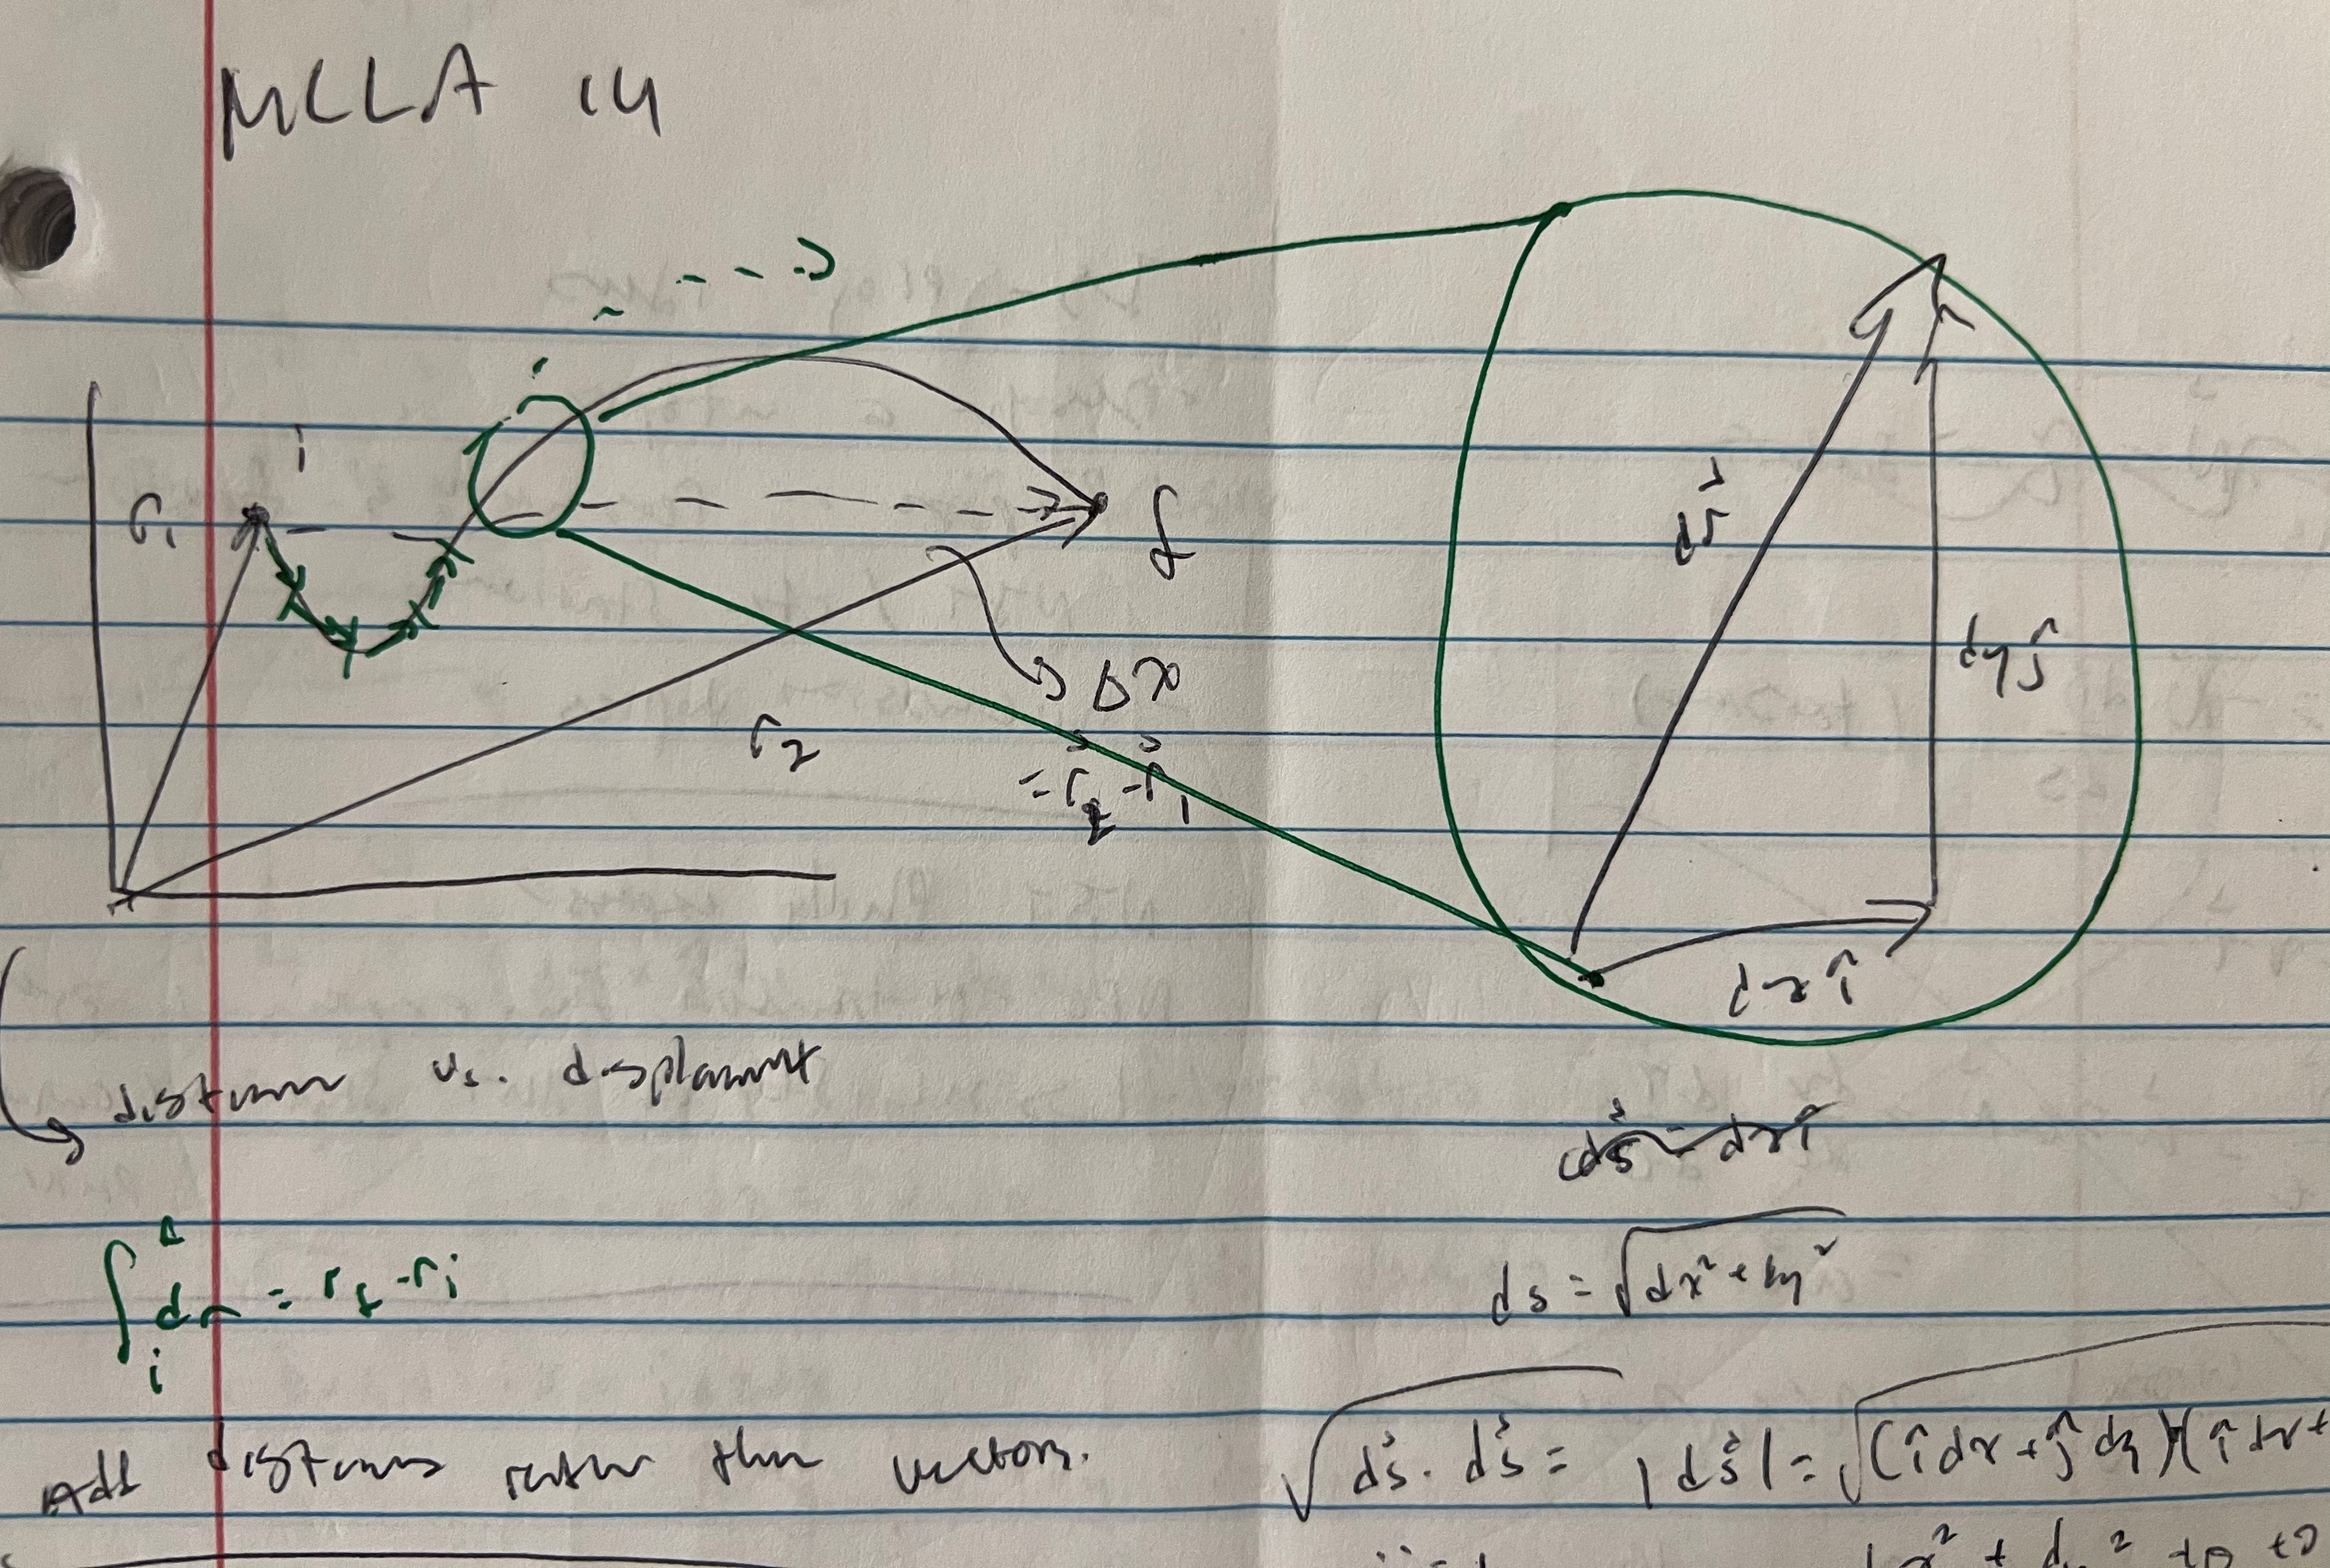
\includegraphics[scale=0.1]{path-length.jpg}
        \1 curvature of a curve is defined as: \[\kappa=\left|\dfrac{d\mathbf T}{ds}\right|\] where $\mathbf T$ is the unit tangent vector. 
        \1 \[\kappa(t)=\dfrac{|\mathbf T'(t)|}{|\mathbf r'(t)|}\]
        \1 The curvature of the curve given by the vector function $\mathbf r$ is \[\kappa(t)=\dfrac{|\mathbf r'(t)\times\mathbf r''(t)|}{|\mathbf r'(t)|^3}\]
        \1 Equations for unit tangent, unit normal and binormal vectors, and curvature: \[\mathbf T(t)=\dfrac{\mathbf r'(t)}{|\mathbf r'(t)|}\qquad \mathbf N(t)=\dfrac{\mathbf T'(t)}{|\mathbf T'(t)|}\qquad \mathbf B(t)=\mathbf T(t)\times\mathbf N(t)\]\[\kappa=\left|\dfrac{d\mathbf T}{ds}\right|=\dfrac{|\mathbf T'(t)|}{|\mathbf r'(t)|}=\dfrac{|\mathbf r'(t)\times r''(t)|}{|\mathbf r'(t)|^3}\]
        \1 Visual representation of the vectors: \\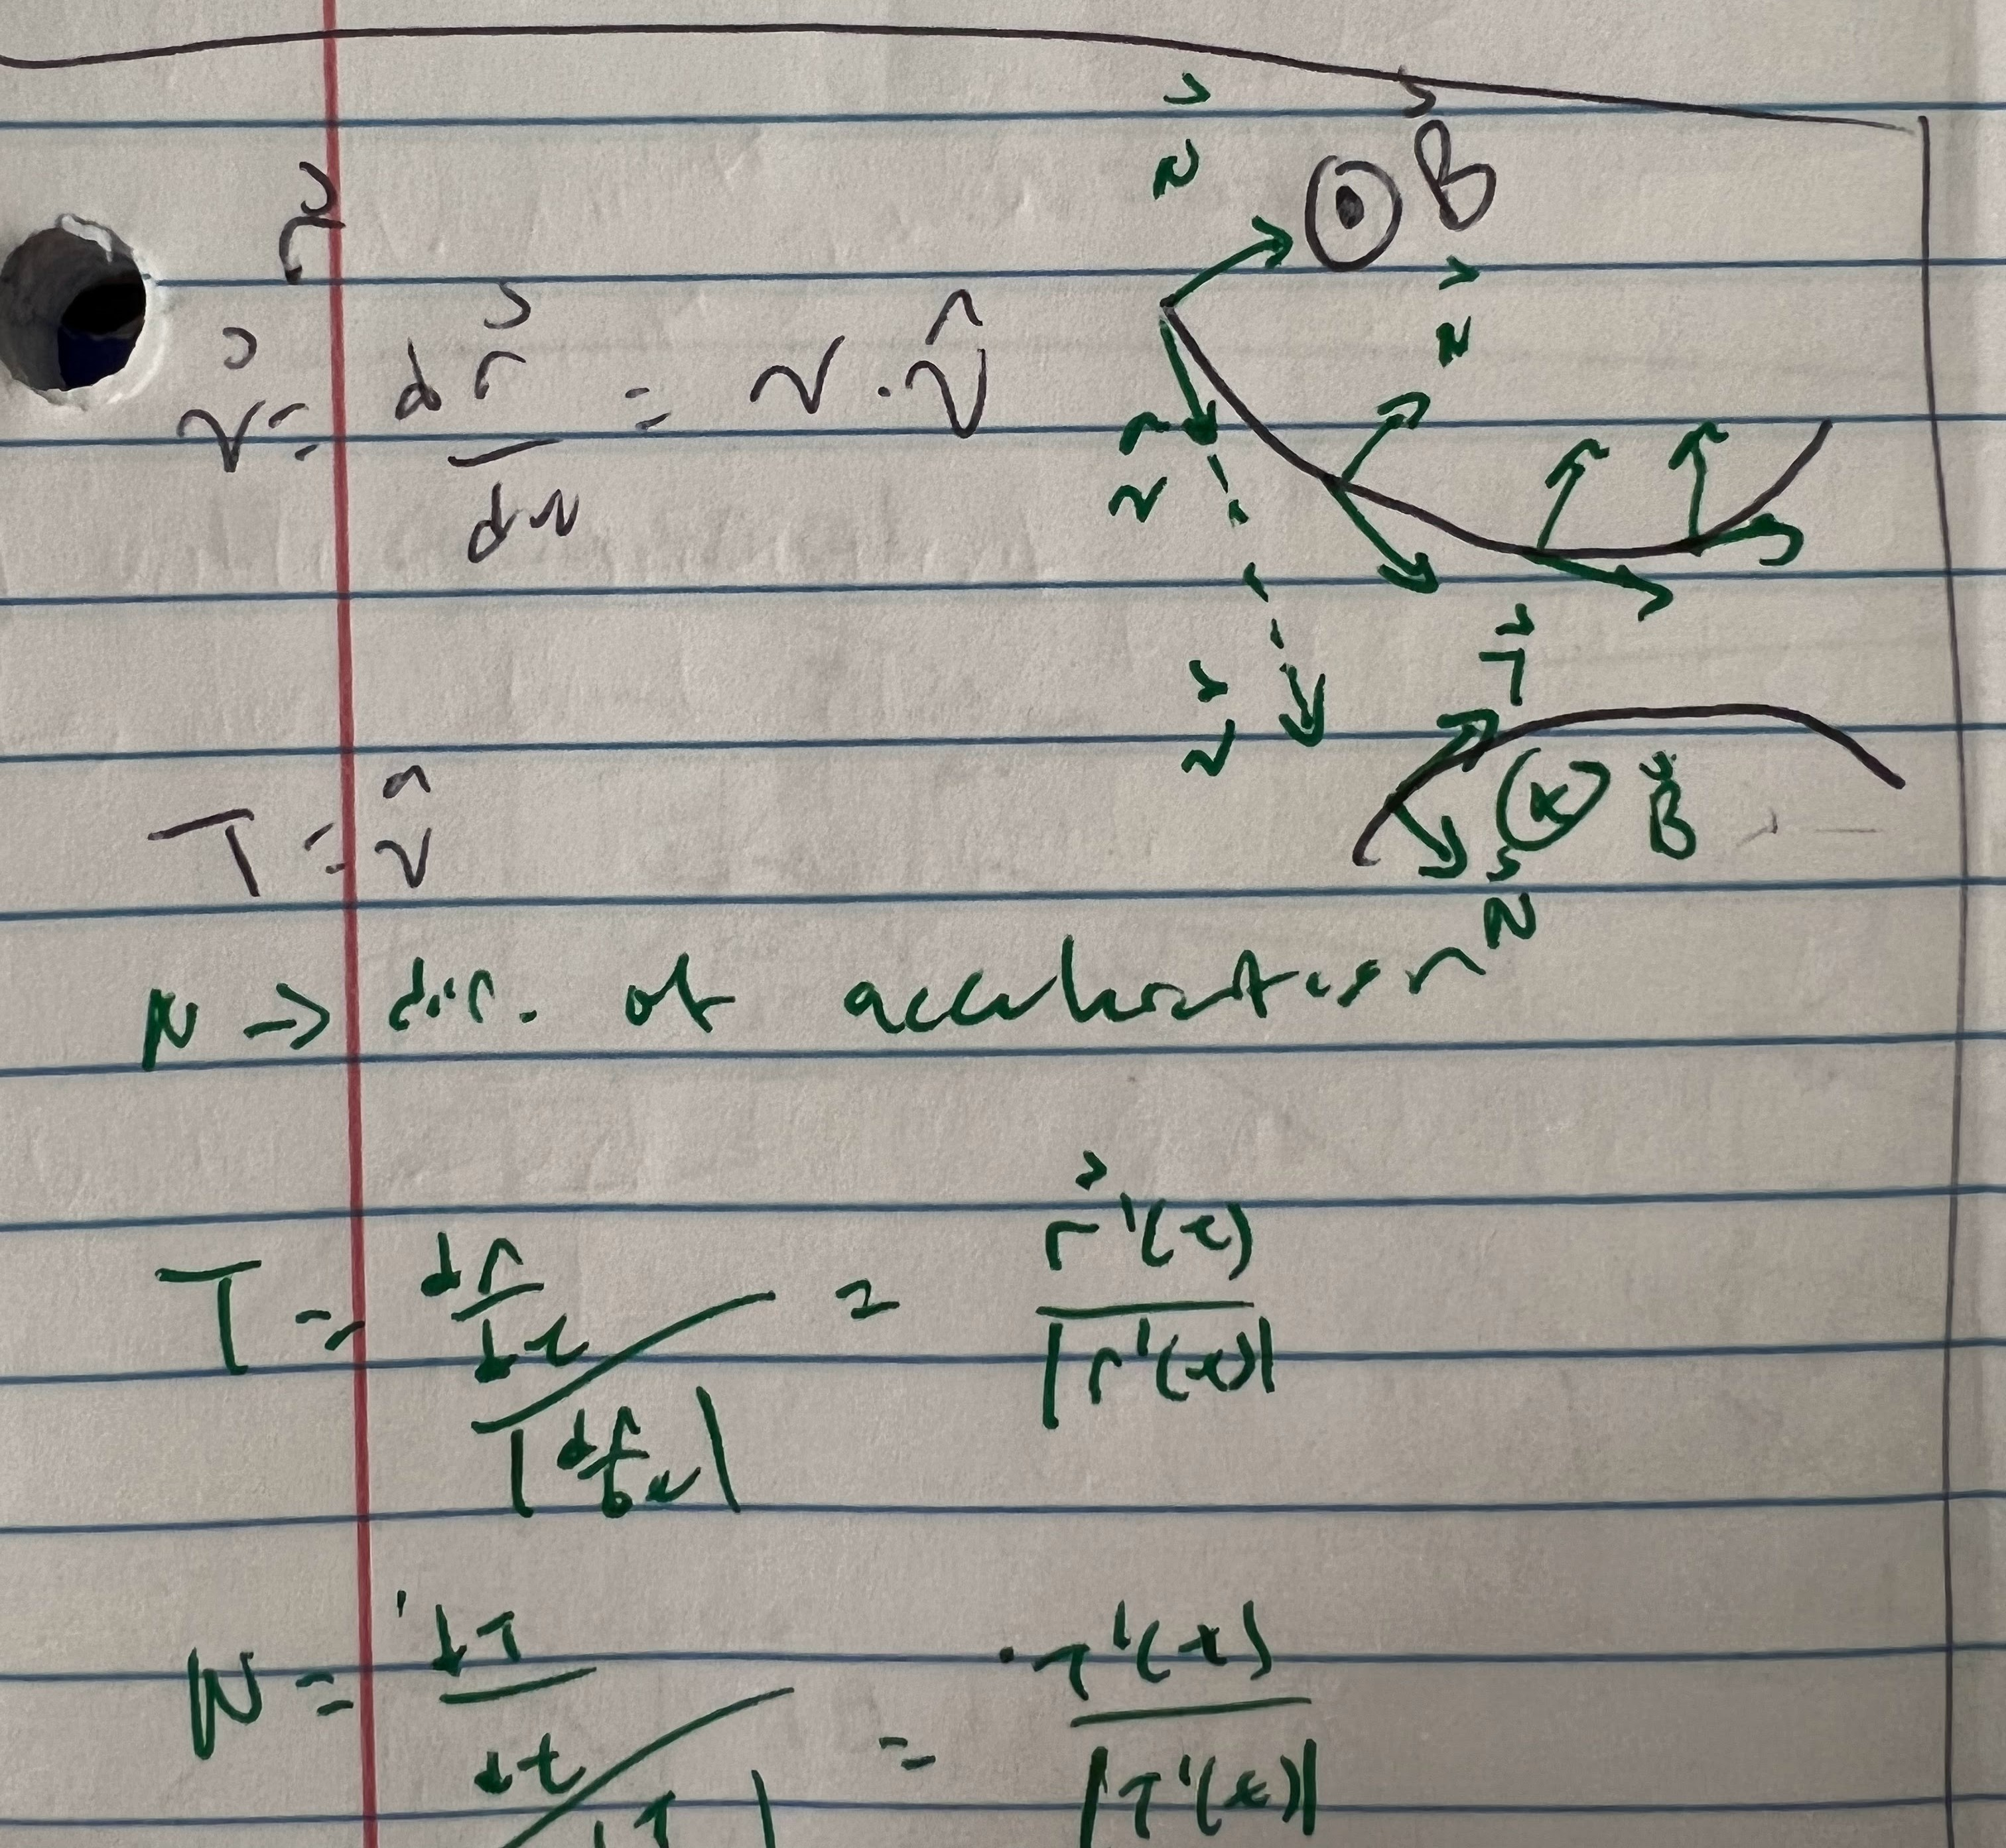
\includegraphics[scale=0.1]{visual-vectors.jpg}
    \end{outline}
    
    \subsection{Motion in Space: Velocity and Acceleration}
    \begin{outline}
        \1 Velocity: \[\mathbf v(t)=\mathbf r'(t)\]
        \1 speed is the magnitude of velocity. 
        \1 Parametric equations of trajectory: \[x=(v_0\cos\alpha)t\qquad y=(v_0\sin\alpha)t-\frac{1}{2}gt^2\]
        \1 Tangential and normal components of acceleration: \[\mathbf a=v'(\mathbf T)+\kappa v^2\mathbf N\]
        \1 Kepler's laws: 
            \2 A planet revolves around the sun in an elliptical orbit with the sun at one focus. 
            \2 The line joining the sun to a planet sweeps out equal areas in equal times. 
            \2 The square of the period of revolution of a planet is proportional to the cube of the length of the major axis of orbit. 
    \end{outline}

    \section{Partial Derivatives} % chapter title
    \subsection{Functions of Several Variables} % section topic
    \begin{outline}
        \1 A function $f$ of two variables is a rule that assigns to each ordered pair of real numbers \((x,y)\) in a set $D$ a unique real number denoted by \(f(x,y)\). The set $D$ is the domain of $f$ and its range is the set of values that $f$ takes on, that is \({f(x,y)|(x,y)\in D}\)
        \1 If $f$ is a function of two variables with domain $D$, then the graph of $f$ is the set of all points \((x,y,z)\) in \(\mathbb{R}^3\) such that \(z=f(x,y)\) and \((x,y)\) is in $D$. 
        \1 The level curves of a function $f$ of two variables are the curves with equations \(f(x,y)=k\), where $k$ is a constant (in the range of $f$). 
            \2 A level curve is the set ofa ll points in the domain of $f$ at which $f$ takes on a given value $k$. (Think of countour maps, equipotential lines)


    \end{outline}
    \subsection{Limits and Continuity}
    \begin{outline}
        \1 Let $f$ be a function of two variables whose domain $D$ includes points arbitrarily close to \((a,b)\). Then we say that the limit of \(f(x,y)\) as \(x,y\) approaches \((a,b)\) is $L$ and we write \[\lim_{(x,y)\to(a,b)}f(x,y)=L\] if for every number \(\varepsilon>0\) there is a corresponding number \(\delta>0\) such that \[\text{if}\qquad(x,y)\in D\qquad\text{and}\qquad 0<\sqrt{(x-a)^2+(y-b)^2}<\delta\qquad\text{then}\qquad|f(x,y)-L|<\varepsilon\]
        \1 If \(f(x,y)\to L_1\) as \((x,y)\to(a,b)\) along a path $C_1$ and \(f(x,y)\to L_2\) as \((x,y)\to(a,b)\) along a path $C_2$, where \(L_1\neq L_2\), then \(\lim_{(x,y)\to(a,b)}f(x,y)\) does not exist. 
        \1 A function $f$ of two variables is called continuous at \((a,b)\) if \[\lim_{(x,y)\to(a,b)f(x,y)=f(a,b)}\] We say $f$ is continuous on $D$ if $f$ is continuous at every point \((a,b)\) in $D$. 
        \1 If $f$ is defined on a subset $D$ of \(\mathbb{R}^n\), then \(\lim_{\mathbf x\to\mathbf a}f(\mathbf x)=L\) means that for every number \(\varepsilon>0\) there is a corresponding number \(\delta>0\) such that \[\text{if}\qquad x\in D\qquad\text{and}\qquad 0<|\mathbf x-\mathbf a|<\delta \qquad\text{then}\qquad |f(\mathbf x)-L|<\varepsilon\]
    \end{outline}
    \subsection{Partial Derivatives}
    \begin{outline}
        \1 If $f$ is a function of two variables, its partial derivatives are the functions $f_x$ and $f_y$ defined by \[f_x(x,y)=\lim_{h\to0}\dfrac{f(x+h,y)-f(x,y)}{h}\]\[f_y(x,y)=\lim_{h\to0}\dfrac{f(x,y+h)-f(x,y)}{h}\]
        \1 If \(z=f(x,y)\), we write \[f_x(x,y)=f_x=\dfrac{\partial f}{\partial x}=\dfrac{\partial}{\partial x}f(x,y)=\dfrac{\partial z}{\partial x}=f_1=D_1f=D_xf\]\[f_y(x,y)=f_y=\dfrac{\partial f}{\partial y}=\dfrac{\partial}{\partial y}f(x,y)=\dfrac{\partial z}{\partial y}=f_2=D_2f=D_yf\]
        \1 Finding partial derivatives of \(z=f(x,y)\):
            \2 To find $f_x$, regard $y$ as a constant and differentiate \(f(x,y)\) with respect to $x$. 
            \2 To find $f_y$, regard $x$ as a constant and differentiate \(f(x,y)\) with respect to $y$. 
        \1 Clairaut's Theorem: suppose $f$ is defined on a disk $D$ that contains the point \((a,b)\). If the functions \(f_{xy}\) and \(f_{yx}\) are both continuous on $D$, then \[f_{xy}(a,b)=f_{yx}(a,b)\]
        \1 3D Laplace Equation: \[\dfrac{\partial^2u}{\partial x^2}+\dfrac{\partial^2u}{\partial y^2}+\dfrac{\partial^2u}{\partial z^2}=0\]

    \end{outline}
    \subsection{Tangent Planes and Linear Approximations}
    \begin{outline}
        \1 Suppose $f$ has continuous partial derivatives. An equation of the tangent plane to the surface \(z=f(x,y)\) at the point \(P(x_0,y_0,z_0)\) is \[z-z_0=f_x(x_0,y_0)(x-x_0)+f_y(x_0,y_0)(y-y_0)\]
        \1 If \(z=f(x,y)\), then $f$ is differentiable at \((a,b)\) if \(\Delta z\) can be expressed in the form \[\Delta z=f_x(a,b)\Delta x+f_y(a,b)\Delta y+\varepsilon_1\Delta x+\varepsilon_2\Delta y\] where \(\varepsilon_1\) and \(\varepsilon_2\to 0\) as \((\Delta x,\Delta y)\to(0,0)\). 
        \1 Theorem: If the partial derivatives \(f_x\) and \(f_y\) exist near \((a,b)\) and are continuous at \((a,b)\), then $f$ is differentiable at \((a,b)\). 
        \1 The total differential $dz$ is defined by: \[dz=f_x(x,y)dx+f_y(x,y)dy=\dfrac{\partial z}{\partial x}dx+\dfrac{\partial z}{\partial y}dy\]

    \end{outline}
    \subsection{The Chain Rule}
    \begin{outline}
        \1 Case 1: suppose that \(z=f(x,y)\) is a differentiable function of $x$ and $y$, where \(x=g(t)\) and \(y=h(t)\) are both differentiable functions of $t$. Then $z$ is a differentiable function of $t$ and \[\dfrac{dz}{dt}=\dfrac{\partial f}{\partial x}\dfrac{dx}{dt}+\dfrac{\partial f}{\partial y}\dfrac{dy}{dt}\] or \[\dfrac{dz}{dt}=\dfrac{\partial z}{\partial x}\dfrac{dx}{dt}+\dfrac{\partial z}{\partial y}\dfrac{dy}{dt}\]
        \1 Case 2: Suppose that \(z=f(x,y)\) is a differentiable function of $x$ and $y$, where \(x=g(s,t)\) and \(y=h(s,t)\) are differentiable functions of $s$ and $t$. Then \[\pdv{z}{s}=\pdv{z}{x}\pdv{x}{s}+\pdv{z}{y}\pdv{y}{s}\qquad\pdv{z}{t}=\pdv{z}{x}\pdv{x}{t}+\pdv{z}{y}\pdv{y}{t}\]
        \1 General Version: Suppose that $u$ is a differentiable function of the $n$ variables \(x_1,x_2,\cdots,x_n\) and each \(x_j\) is a differentiable function of the $m$ variables \(t_1,t_2,\cdots,t_m\). Then $u$ is a function of \(t_1,t_2,\cdots,t_m\) and \[\pdv{u}{t_i}=\pdv{u}{x_1}\pdv{x_1}{t_i}+\pdv{u}{x_2}\pdv{x_2}{t_i}+\cdots+\pdv{u}{x_n}\pdv{x_n}{t_i}\] for each \(i=1,2,\cdots,m\)
        \1 Implicit diffentiation: \[\dfrac{dy}{dx}=-\dfrac{\pdv{F}{x}}{\pdv{F}{y}}=-\dfrac{F_x}{F_y}\] where \(y=f(x)\) and \(F(x,f(x))=0\)
        \1 \[\pdv{z}{x}=-\dfrac{\pdv{F}{x}}{\pdv{F}{z}}\qquad\pdv{z}{y}=-\dfrac{\pdv{F}{y}}{\pdv{F}{z}}\]


    \end{outline}
    \subsection{Directional Derivatives and the Gradient Vector}
    \begin{outline}
        \1 The directional derivative of $f$ at \((x_0,y_0)\) in the direction of a unit vector \(\vb{u}=\langle a,b\rangle \) is \[D_{\vb{u}}f(x_0,y_0)=\lim_{h\to 0}\dfrac{f(x_0+ha,y_0+hb)-f(x_0,y_0)}{h}\] if this limit exists. 
        \1 Theorem: If $f$ is a differentiable function of $x$ and $y$, then $f$ has a directional derivative in the direction of any unit vector \(\vb{u}=\langle a,b\rangle\) and \[D_{\vb{u}}f(x,y)=f_x(x,y)a+f_y(x,y)b\]
            \2 If the unit vector \(\vb{u}\) makes an angle \(\theta\) with the positive $x$-axis, then we can write \(\vb{u}=\langle\cos\theta,\sin\theta\rangle\) and the previous eqn becomes: \[D_{\vb{u}}f(x,y)=f_x(x,y)\cos\theta+f_y(x,y)\sin\theta\]
        \1 If $f$ is a function of two variables $x$ and $y$, then the gradient of $f$ is the vector function \(\grad{f}\) defined by \[\grad{f(x,y)}=\langle f_x(x,y),f_y(x,y)\rangle=\pdv{f}{x}\vb{i}+\pdv{f}{y}\vb{j}\]
        \1 The equation of the directional derivative of a differentiable function can thus be written as: \[D_{\vb{u}}f(x,y)=\grad{f(x,y)}\cdot\vb{u}\]
        \1 The directional derivative of $f$ at \((x_0,y_0,z_0)\) in the direction of a unit vector \(\vb{u}=\langle a,b,c\rangle\) is \[D_{\vb{u}}f(x_0,y_0,z_0)=\lim_{h\to 0}\dfrac{f(x_0+ha,y_0+hb,z_0+hc)-f(x_0,y_0,z_0)}{h}\] if this limit exists. 
        \1 Using vector notation: \[D_{\vb{u}}f(\vb{x}_0)=\lim_{h\to 0}\dfrac{f(\vb{x_0}+h\vb{u})-f(\vb{x}_0)}{h}\]
        \1 For a function of three variables, the gradient vector: \[\grad{f}=\langle f_x,f_y,f_z\rangle=\pdv{f}{x}\vb{i}+\pdv{f}{y}\vb{j}+\pdv{f}{z}\vb{k}\]
        \1 The directional derivative of a function of three variables: \[D_{\vb{u}}f(x_0,y_0,z_0)=\grad{f(x,y,z)\cdot\vb{u}}\]
        \1 Theorem: Suppose $f$ is a differentiable function of two or three variables. The maximum value of the directional derivative \(D_{\vb{u}}f(\vb{x})\) is \(|\grad f(\vb{x})|\) and it occurs when \(\vb{u}\) has the same direction as the gradient vector \(\grad f(\vb{x})\). 
        \1 The tangent plane to a level surface \(F(x,y,z)=k\) at \(P(x_0,y_0,z_0)\) is the plane that passes through $P$ and has normal vector \(\grad F(x_0,y_0,z_0)\). The equation of the tangent plane is thus: \[F_x(x_0,y_0,z_0)(x-x_0)+F_y(x_0,y_0,z_0)(y-y_0)+F_z(x_0,y_0,z_0)(z-z_0)=0\]
        \1 The normal line to the surface $S$ at $P$ is the line passing through $P$ and perpendicular to the tangent plane. The direction of the normal line is therefore given by the gradient vector \(\grad F(x_0,y_0,z_0)\); its symmetric equations are given by: \[\dfrac{x-x_0}{F_x(x_0,y_0,z_0)}=\dfrac{y-y_0}{F_y(x_0,y_0,z_0)}=\dfrac{z-z_0}{F_z(x_0,y_0,z_0)}\]

    \end{outline}
    
        
    \subsection{Maximum and Minimum Values}
    \begin{outline}
        \1 A function of two variables has a local maximum at \((a,b)\) if \(f(x,y)\leq f(a,b)\) when \((x,y)\) is near \((a,b)\). [This means that \(F(x,y)\leq f(a,b)\) for all points \((x,y)\) in some disk with center \((a,b)\).] The number \(f(a,b)\) is called a local maximum value. If \(f(x,y)\geq f(a,b)\) when \((x,y)\) is near \((a,b)\), then $f$ has a local minimum at \((a,b)\) and \(f(a,b)\) is a local minimum value. 
        \1 Theorem: If $f$ has a local maximum or minimum at \((a,b)\) and the first order partial derivatives of $f$ exist there, then \(f_x(a,b)=0\) and \(f_y(a,b)=0\). 
        \1 Second derivatives test: Suppose the second partial derivatives of $f$ are continuous on a disk with center \((a,b)\), and suppose that \(f_x(a,b)=0\) and \(f_y(a,b)=0\) [that is, \((a,b)\) is a critical point of $f$]. Let \[D=D(a,b)=f_{xx}(a,b)f_{yy}(a,b)-[f_{xy}(a,b)]^2\]
            \2 If \(D>0\) and \(f_{xx}(a,b)>0\), then \(f(a,b)\) is a local minimum. 
            \2 If \(D>0\) and \(f_{xx}(a,b)<0\), then \(f(a,b)\) is a local maximum. 
            \2 If \(D<0\), the \(f(a,b)\) is not a local maximum or minimum. 
        \1 Extreme value theorem for functions of two variables: If $f$ is continuous on a closed, bounded set $D$ in \(\mathbb{R}^2\), then $f$ attains an absolute maximum value \(f(x_1,y_1)\) and an absolute minimum value \(f(x_2,y_2)\) at some points \((x_1,y_1)\) and \((x_2,y_2)\) in $D$. 
        \1 To find the absolute maximum and minimum values of a continuous function $f$ on a closed, bounded set $D$:
    \0 
        \begin{enumerate}
            \item Find the values of $f$ at the critical points of $f$ in $D$. 
            \item Find the extreme values of $f$ on the boundary of $D$. 
            \item The largest of the values from steps one and 2 is the absolute maximum value; the smallest of these values is the absolute minimum value. 
        \end{enumerate}

    \end{outline}
    \subsection{Lagrange Multipliers}
    \begin{outline}
        \1 Method of Lagrange Multipliers: To find the maximum and minimum values of \(f(x,y,z)\) subject to the constraint \(g(x,y,z)=k\) [assuming that these extreme values exist and \(\grad{g}\neq \vb{0}\) on the surface \(g(x,y,z)=k\)]: 
        \begin{enumerate}
            \item Find all values of \(x,y,z\), and \(\lambda\) such that \[\grad f(x,y,z)=\lambda\grad g(x,y,z)\] and \[g(x,y,z)=k\]
            \item Evaluate $f$ at all the points \((x,y,z)\) that result from step 1. The largest of these values is the maximum value of $f$; the smallest is the minimum value of $f$. 
        \end{enumerate}

    \end{outline}

\begin{outline}
        \1 With two constraints, \(g(x,y,z)=k\) and \(h(x,y,z)=c\), there exist Lagrange Multipliers, constants \(\lambda\) and \(\mu\) such that \[\grad f(x_0,y_0,z_0)=\lambda\grad g(x_0,y_0,z_0)+\mu\grad h(x_0,y_0,z_0)\]
    \end{outline}

    \section{Multiple Integrals} % chapter title
    \subsection{Double Integrals over Rectangles} % section topic
    \begin{outline}
        \1 The double integral of $f$ over the rectangle $R$ is \[\iint\limits_Rf(x,y)dA=\lim_{m,n\to\infty}\sum^m_{i=1}\sum^n_{j=1}f(x_{ij}^*,y_{ij}^*)\Delta A\] if this limit exists. 
        \1 If \(f(x,y)\geq 0\), then the volume $V$ of the solid that lies above the rectangle $R$ and below the surface \(z=f(x,y)\) is \[V=\iint\limits_Rf(x,y)dA\]
        \1 Midpoint rule for double integrals: \[\iint\limits_Rf(x,y)dA\approx\sum^m_{i=1}\sum^n_{j=1}f(\bar x_i,\bar y_j)\Delta A\] where \(\bar x_i\) is the midpoint of \([x_{i-1},x_i]\) and \(\bar y_j\) is the midpoint of \([y_{j-1},y_j]\). 
        \1 Fubini's Theorem: If $f$ is continuous on the rectangle \(R=\{(x,y)\;|\;a\leq x\leq b,c\leq y\leq d\}\), then \[\iint\limits_Rf(x,y)dA=\int^b_a\int^d_cf(x,y)dydx=\int^d_c\int^b_af(x,y)dxdy\] More generally, this is true if we assume that $f$ is bounded on $R$, $f$ is discontinuous only on a finite number of smooth curves, and the iterated integrals exist. 
        \1 \[\iint\limits_Rg(x)h(y)dA=\int^b_ag(x)dx\int^d_ch(y)dy\qquad\text{where }R=[a,b]\times[c,d]\]

    \end{outline}
    \subsection{Double Integrals over General Regions}
    \begin{outline}
        \1 If $F$ is integrable over $R$, then we define the double integral of $f$ over $D$ by \[\iint\limits_Df(x,y)dA=\iint\limits_RF(x,y)dA\qquad\text{where }F\text{ is given by Equation 1}\]
        \1 If $f$ is continuous on a type I region $D$ such that \[D=\{(x,y)\;|\;a\leq x\leq b, g_1(x)\leq y\leq g_2(x)\}\] then \[\iint\limits_Df(x,y)dA=\int^b_a\int^{g_2(x)}_{g_1(x)}f(x,y)dydx\]
        \1 Type II plane regions: \[D=\{(x,y)\;|\;c\leq y\leq d, h_1(y)\leq x\leq h_2(y)\}\]
        \1 If $D$ is a type II region, \[\iint\limits_Df(x,y)dA=\int^d_c\int^{h_2(y)}_{h_1(y)}f(x,y)dxdy\]
        \1 Properties of double integrals 
            \2 \[\iint\limits_D[f(x,y)+g(x,y)]dA=\iint\limits_Df(x,y)dA+\iint\limits_Dg(x,y)dA\]
            \2 \[\iint\limits_Dcf(x,y)dA=c\iint\limits_Df(x,y)dA\] where $c$ is a constant
            \2 If \(f(x,y)\geq g(x,y)\) for all \((x,y)\) in $D$, then \[\iint\limits_Df(x,y)dA\geq\iint\limits_Dg(x,y)dA\]
        \1 If \(D=D_1\cup D_2\), where $D_1$ and $D_2$ don't overlap except perhaps on their boundaries, then \[\iint\limits_Df(x,y)dA=\iint\limits_{D_1}f(x,y)dA+\iint\limits_{D_2}f(x,y)dA\]
        \1 \[\iint\limits_D1dA=A(D)\]
        \1 If \(m\leq f(x,y)\leq M\) for all \((x,y)\) in $D$, then \[mA(D)\leq\iint\limits_Df(x,y)dA\leq MA(D)\]
    \end{outline}
    \subsection{Double Integrals in Polar Coordinates}
    \begin{outline}
        \1 Recall: \[r^2=x^2+y^2\qquad\qquad x=r\cos\theta\qquad\qquad y=r\sin\theta\]
        \1 Change to polar coordinates in a double integral: If $f$ is continuous on a polar rectangle $R$ given by \(0\leq a\leq r\leq b,\alpha\leq\theta\leq\beta\), where \(0\leq\beta-\alpha\leq2\pi\), then \[\iint\limits_Rf(x,y)dA=\int^\beta_\alpha\int^b_af(r\cos\theta,r\sin\theta)rdrd\theta\]
        \1 If $f$ is continuous on a polar region of the form \[D=\{(r,\theta)\;|\;\alpha\leq\theta\leq\beta,h_1(\theta)\leq r\leq h_2(\theta)\}\] then \[\iint\limits_Df(x,y)dA=\int^\beta_\alpha\int^{h_2(\theta)}_{h_1(\theta)}f(r\cos\theta,r\sin\theta)rdrd\theta\]
    \end{outline}
    \subsection{Applications of Double Integrals}
    \begin{outline}
        \1 mass of a lamina: \[m=\lim_{k,l\to\infty}\sum^k_{i=1}\sum^l_{j=1}\rho(x^*_{ij},y^*_{ij})\Delta A=\iint\limits_D\rho(x,y)dA\]
        \1 Total charge in a given area: \[Q=\iint\limits_D\sigma(x,y)dA\]
        \1 Moment of a lamina about the $x$ axis: \[M_x=\lim_{m,n\to\infty}\sum^m_{i=1}\sum^n_{j=1}y^*_{ij}\rho(x^*_{ij},y^*_{ij})\Delta A=\iint\limits_D\rho(x,y)dA\]
        \1 About the $y$ axis: \[M_y=\lim_{m,n\to\infty}\sum^m_{i=1}\sum^n_{j=1}x^*_{ij}\rho(x^*_{ij},y^*_{ij})\Delta A=\iint\limits_Dx\rho(x,y)dA\]
        \1 The coordinates \((\bar x,\bar y)\) of the center of mass of a lamina occupying the region $D$ and having density function \(\rho(x,y)\) are \[\bar x=\dfrac{M_y}{m}=\dfrac{1}{m}\iint\limits_Dx\rho(x,y)dA\qquad\qquad\bar y=\dfrac{M_x}{m}=\dfrac{1}{m}\iint\limits_Dy\rho(x,y)dA\] where the mass $m$ is given by \[m=\iint\limits_D\rho(x,y)dA\]
        \1 Moment of intertia about $x$ axis: \[I_x=\lim_{m,n\to\infty}\sum^m_{i=1}\sum^n_{j=1}(y^*_{ij})^2\rho(x^*_{ij},y^*_{ij})\Delta A=\iint\limits_Dy^2\rho(x,y)dA\]
        \1 About the $y$ axis: \[I_y=\lim_{m,n\to\infty}\sum^m_{i=1}\sum^n_{j=1}(x^*_{ij})^2\rho(x^*_{ij},y^*_{ij})\Delta A=\iint\limits_Dx^2\rho(x,y)dA\]
        \1 Moment of inertia about the origin, or polar moment of intertia: \[I_0=\lim_{m,n\to\infty}\sum^m_{i=1}\sum^n_{j=1}\left[(x^*_{ij})^2+(y^*_{ij})^2\right]\rho(x^*_{ij},y^*_{ij})\Delta A=\iint\limits_D(x^2+y^2)\rho(x,y)dA\] where \(I_0=I_x+I_y\)
        \1 Radius of gyration of a lamina about an axis is the number $R$ such that \[mR^2=I\]
        \1 Radius of gyration \(\overline{\overline{y}}\) with respect to $x$ axis and radius of gyration \(\overline{\overline{x}}\) with respect to the $y$ axis are given by \[m\overline{\overline{y}}^2=I_x\qquad\qquad m\overline{\overline{x}}^2=I_y\]
        \1 Expected values: if $X$ and $Y$ are random variables with joint density function $f$, we defined the $X$-mean and $Y$-mean, or expected values of $X$ and $Y$ as \[\mu_1=\iint\limits_{\mathbb R^2}xf(x,y)dA\qquad\qquad\mu_2=\iint\limits_{\mathbb R^2}yf(x,y)dA\]
        \1 A single random variable is normally distributed if its probability density function is of the form \[f(x)=\dfrac{1}{\sigma\sqrt{2\pi}}e^{-(x-\mu)^2/(2\sigma^2)}\] where \(\mu\) is the mean and \(\sigma\) is the standard deviation. 
    \end{outline}
    \subsection{Surface Area}
    \begin{outline}
        \1 The surface area of a surface $S$ is \[A(S)=\lim_{m,n\to\infty}\sum^m_{i=1}\sum^n_{j=1}\Delta T_{ij}\]
        \1 The area of the surface with equation \(z=f(x,y),(x,y)\in D\), where \(f_x\) and \(f_y\) are continuous, is \[A(S)=\iint\limits_D\sqrt{[f_x(x,y)]^2+[f_y(x,y)]^2+1}dA\] which is also \[A(S)=\iint\limits_D\sqrt{1+\left(\pdv{z}{x}\right)^2+\left(\pdv{z}{y}\right)^2}dA\]

    \end{outline}
    \subsection{Triple Integrals}
    \begin{outline}
        \1 The triple integral of $f$ over the box $B$ is \[\iiint\limits_Bf(x,y,z)dV=\lim_{l,m,n\to\infty}\sum^l_{i=1}\sum^m_{j=1}\sum^n_{k=1}f(x^*_{ijk},y^*_{ijk},z^*_{ijk})dV\] if this limit exists. 
        \1 If we choose the sample point to be \((x_i,y_j,z_k)\), we get \[\iiint\limits_Bf(x,y,z)dV=\lim_{l,m,n\to\infty}\sum^l_{i=1}\sum^m_{j=1}\sum^n_{k=1}f(x_i,y_j,z_k)\Delta V\]
        \1 Fubini's theorem for triple integrals: If $f$ is continuous on the rectangular box \(B=[a,b]\times[c,d]\times[r,s]\),  then \[\iiint\limits_Bf(x,y,z)dV=\int^s_r\int^d_c\int^b_af(x,y,z)dxdydz\]
        \1 A solid region $E$ is said to be of type 1 if it lies between the graphs of two continuous functions of $x$ and $y$, that is, \[E=\{(x,y,z)\;|\;(x,y)\in D, u_1(x,y)\leq z\leq u_2(x,y)\}\]
        \1 If $E$ is a type 1 region: \[\iiint\limits_Ef(x,y,z)dV=\iint\limits_D\left[\int^{u_2(x,y)}_{u_1(x,y)}f(x,y,z)dz\right]dA\]
        \1 If the projection of $D$ of $E$ onto the $xy$ plane is a type I plane region, then \[E=\{(x,y,z)\;|\;a\leq x\leq b, g_1(x)\leq y\leq g_2(x), u_1(x,y)\leq z\leq u_2(x,y)\}\], and \[\iiint\limits_Ef(x,y,z)dV=\int^b_a\int^{g_2(x)}_{g_1(x)}\int^{u_2(x,y)}_{u_1(x,y)}f(x,y,z)dzdydx\]
        \1 If $D$ is a type II plane region, then \[E=\{(x,y,z)\;|\;c\leq y\leq d, h_1(y)\leq x \leq h_2(y),u_1(x,y)\leq z\leq u_2(x,y)\}\], and \[\iiint\limits_Ef(x,y,z)dV=\int_c^d\int_{h_1(y)}^{h_2(y)}\int_{u_1(x,y)}^{u_2(x,y)}f(x,y,z)dzdxdy\]
        \1 A solid region $E$ is of type 2 if: \[E=\{(x,y,z)\;|\;(y,z)\in D,u_1(y,z)\leq x\leq u_2(y,z)\}\] where $D$ is the projection of $E$ onto the $yz$ plane. The back surface is \(x=u_1(y,z)\) and the front surface is \(x=u_2(y,z)\), and \[\iiint\limits_Ef(x,y,z)dV=\iint\limits_D\left[\int_{u_1(y,z)}^{u_2(y,z)}f(x,y,z)dx\right]dA\]
        \1 A type 3 region is of the form: \[E=\{(x,y,z)\;|\;(x,z)\in D, u_1(x,z)\leq y\leq u_2(x,z)\}\] where $D$ is the projection of $E$ onto the $xz$ plane, \(y=u_1(x,z)\) is the left surface, and \(y=u_2(x,z)\) is the right surface. Thus, \[\iiint\limits_Ef(x,y,z)dV=\iint\limits_D\left[\int_{u_1(x,z)}^{u_2(x,z)}f(x,y,z)dy\right]dA\]
        \1 If \(f(x,y,z)=1\) for all points in $E$, then: \[V(E)=\iiint\limits_EdV\]
    \end{outline}
    \subsection{Triple Integrals in Cylindrical Coordinates}
    \begin{outline}
        \1 Recall: \[r^2=x^2+y^2\qquad\qquad x=r\cos\theta\qquad\qquad y=r\sin\theta\qquad\qquad z=z\qquad\qquad\tan\theta=\dfrac{y}{x}\]
        \1 Triple integration in cylindrical coordinates: \[\iiint\limits_Ef(x,y,z)dV=\int_\alpha^\beta\int_{h_1(\theta)}^{h_2(\theta)}\int_{u_1(r\cos\theta,r\sin\theta)}^{u_2(r\cos\theta,r\sin\theta)}f(r\cos\theta,r\sin\theta,z)rdzdrd\theta\]

    \end{outline}
    \subsection{Triple Integrals in Spherical Coordinates}
    \begin{outline}
        \1 Recall: \[x=\rho\sin\phi\cos\theta\qquad\qquad y=\rho\sin\phi\sin\theta\qquad\qquad z=\rho\cos\phi \qquad\qquad\rho^2=x^2+y^2+z^2\]
        \1 Triple integral in spherical coordinates: \[\iiint\limits_Ef(x,y,z)dV=\int^d_c\int^\beta_\alpha\int^b_af(\rho\sin\phi\cos\theta,\rho\sin\phi\sin\theta,\rho\cos\phi)\rho^2\sin\phi d\rho d\theta d\phi\] where $E$ is a spherical wedge given by \[E=\{(\rho,\theta,\phi)\;|\; a\leq\rho\leq b,\alpha\leq\theta\leq\beta, c\leq\phi\leq d\}\]

    \end{outline}
    \subsection{Change of Variables in Multiple Integrals}
    \begin{outline}
        \1 We can write the substitution rule as: \[\int_a^bf(x)dx=\int_c^df(g(u))g'(u)du\] where \(x=g(u)\) and \(a=g(c),b=g(d)\) which is also \[\int_a^bf(x)dx=\int_c^df(x(u))\dfrac{dx}{du}du\]
        \1 The Jacobian of the transformation $T$ given by \(x=g(u,v)\) and \(y=h(u,v)\) is \[\pdv{(x,y)}{(u,v)}=\begin{vmatrix}
            \pdv{x}{u} & \pdv{x}{v} \\\\ \pdv{y}{u} & \pdv{y}{v}
        \end{vmatrix} = \pdv{x}{u}\pdv{y}{v}-\pdv{x}{v}\pdv{y}{u}\]
        \1 Approximation to the area \(\Delta A\) of $R$: \[\Delta A\approx\left|\pdv{(x,y)}{(u,v)}\right|\Delta u\Delta v\] where the Jacobian is evaluated at \((u_0,v_0)\)
        \1 Change of variables in a double integral: Suppose that $T$ is a \(C^1\) transformation whole Jacobian is nonzero and that $T$ maps a region $S$ in the \(uv\) plane onto a region $R$ in the \(xy\) plane. Suppose that $f$ is continuous on $R$ and that $R$ and $S$ are type I or type II plane regions. Suppose also that $T$ is one-to-one, except perhaps on the boundary of $S$. Then: \[\iint\limits_Rf(x,y)dA=\iint\limits_Sf(x(u,v)y(u,v))\left|\pdv{(x,y)}{(u,v)}\right|dudv\]
        \1 If: \[x=g(u,v,w)\qquad\qquad y=h(u,v,w)\qquad\qquad z=k(u,v,w)\] then the Jacobian of $T$ is given by: \[\pdv{(x,y,z)}{{u,v,w}}=\begin{vmatrix}
            \pdv{x}{u} & \pdv{x}{v} & \pdv{x}{w} \\\\ \pdv{y}{u} & \pdv{y}{v} & \pdv{y}{w} \\\\ \pdv{z}{u} & \pdv{z}{v} & \pdv{z}{w}
        \end{vmatrix}\]
        \1 Change of variables for triple integrals: \[\iiint\limits_Rf(x,y,z)dV=\iiint\limits_Sf(x(u,v,w),y(u,v,w),z(u,v,w))\left|\pdv{(x,y,z)}{(u,v,w)}\right| dudvdw\]
        
    \end{outline}

    \section{Vector Calculus} % chapter title
    
        

    \subsection{Vector Fields} % section topic
    \begin{outline}
        \1 Def: Let $D$ be a set in \(\mathbb R^2\) (a plane region). A vector field on \(\mathbb R^2\) is a function \(\vb F\) that assigns to each point \((x,y)\) in $D$ a two-dimensional vector \(\vb F(x,y)\)
        \1 Def: Let $E$ be a subset of \(\mathbb R^3\). A vector field on \(\mathbb R^3\) is a function \(\vb F\) that assigns to each point \((x,y,z)\) in $E$ a three-dimensional vector \(\vb F(x,y,z)\)
        \1 Recall that the gradient of a scalar function $f$ of two variables \(\grad f\) is defined by \[\grad f(x,y)=\pdv{f}{x}\vb i+\pdv{f}{y}\vb j\] Therefore \(\grad f\) is really a vector field on \(\mathbb R^2\) and is called a gradient vector field. Likewise, if $f$ is a scalar function of 3 variables, its gradient is a vector field on \(\mathbb R^3\) given by \[\grad f(x,y,z)=f_x(x,y,z)\vb i+f_y(x,y,z)\vb j+f_z(x,y,z)\vb k\]
        
    \end{outline}    
    \subsection{Line Integrals}
    \begin{outline}
        \1 Def: if $f$ is defined on a smooth curve $C$ given by \[x=x(t)\qquad\qquad y=y(t)\qquad\qquad a\leq t\leq b\] then the line integral of $f$ along $C$ is \[\int_Cf(x,y)ds=\lim_{n\to\infty}\sum^n_{i=1}f(x^*_i,y^*_i)\Delta s_i\] if this limit exists. 
        \1 If $f$ is a continuous function, then the limit always exists and the line integral is given by: \[\int_Cf(x,y)ds=\int^b_af(x(t),y(t))\sqrt{\left(\dfrac{dx}{dt}\right)^2+\left(\dfrac{dy}{dt}\right)^2}dt\] The value of the line integral does not depend on the parameterization of the curve, provided that the curve is traversed exactly once as $t$ increases from $a$ to $b$. 
        \1 Line integrals of $f$ along $C$ with respect to $x$ and $y$: \[\int_Cf(x,y)dx=\lim_{n\to\infty}\sum^n_{i=1}f(x^*_i,y^*_i)\Delta x_i=\int_a^bf(x(t),y(t))x'(t)dt\] \[\int_Cf(x,y)dy=\lim_{n\to\infty}\sum^n_{i=1}f(x^*_i,y^*_i)\Delta y_i=\int_a^bf(x(t),y(t))y'(t)dt\]
        \1 Recall that the vector representation of the line segment that starts at \(\vb r_0\) and ends at \(\vb r_1\) is given by \[\vb r(t)=(1-t)\vb r_0+t\vb r_1\qquad\qquad 0\leq t\leq 1\]
        \1 For line integrals in space, where $C$ is a curve given by \[x=x(t)\qquad\qquad y=y(t)\qquad\qquad z=z(t)\qquad\qquad a\leq t\leq b\] or \[\vb r(t)=x(t)\vb i+y(t)\vb j+z(t)\vb k\] then the line integral of $f$ along $C$ is given by \[\int_Cf(x,y,z)ds=\lim_{n\to\infty}\sum^n_{i=1}f(x^*_i,y^*_i,z^*_i)\Delta s_i=\int_a^bf(x(t),y(t),z(t))\sqrt{\left(\dfrac{dx}{dt}\right)^2+\left(\dfrac{dy}{dt}\right)^2+\left(\dfrac{dz}{dt}\right)^2}dt\]
        \1 We evaluate integrals of the form \[\int_CP(x,y,z)dx+Q(x,y,z)dy+R(x,y,z)dz\] by expressing everything \((x,y,z,dx,dy,dz)\) in terms of the parameter $t$. 
        \1 Def: Let \(\vb F\) be a continuous vector field defined on a smooth curve $C$ given by a vector function \(\vb r(t),a\leq t\leq b\). Then the line integral of $\vb F$ along $C$ is \[\int_C\vb F\cdot d\vb r=\int_a^b\vb F(\vb r(t))\cdot\vb r'(t)dt=\int_C\vb F\cdot\vb Tds\]
        \1 We have: \[\int_C\vb F\cdot d\vb r=\int_CPdx+Qdy+Rdz\qquad\qquad\text{where}\quad\vb F=P\vb i+Q\vb j+R\vb k\]

    \end{outline}
    

    \subsection{The Fundamental Theorem for Line Integrals}
    \begin{outline}
        \1 Theorem: Let $C$ be a smooth curve given by the vector function \(\vb r(t),a\leq t\leq b\). Let $f$ be a differentiable function of two or three variables whos gradient vector \(\grad f\) is continuous on $C$. Then \[\int_C\grad f\cdot d\vb r=f(\vb r(b))-f(\vb r(a))\]
        \1 Theorem: \(\int_C\vb F\cdot d\vb r\) is an independent path in $D$ IFF \(\int_C\vb F\cdot d\vb r=0\) for every closed path $C$ in $D$. 
        \1 Theorem: Suppose \(\vb F\) is a vector field that is continuous on an open connected region $D$. If \(\int_C\vb F\cdot d\vb r\) is independent of path in $D$, then \(\vb F\) is a conservative vector field on $D$; that is, there exists a function $f$ such that \(\grad f=\vb F\)
        \1 Theorem: If \(\vb F(x,y)=P(x,y)\vb i+Q(x,y)\vb j\) is a conservative vector field, where $P$ and $Q$ have continuous first-order partial derivatives on a domain $D$, then throughout $D$ we have \[\pdv{P}{y}=\pdv{Q}{x}\]
        \1 Theorem: Let \(\vb F=P\vb i+Q\vb j\) be a vector field on an open simply-connected region $D$. Suppose that \(P\) and $Q$ have continuous first-order partial derivatives and \[\pdv{P}{y}=\pdv{Q}{x}\qquad\qquad\text{throughout }D\]
    \end{outline}    
    \subsection{Green's Theorem}
    \begin{outline}
        \1 Green's Theorem gives the relationship b/w a line integral around a simple closed curve $C$ and a double integral over the plane region $D$ bounded by $C$. 
        \1 We use the convention that the positive orientation of $C$ means traversing $C$ once counterclockwise. 
        \1 Green's Theorem: Let $C$ be a positively oriented, piecewise-smooth, simple closed curve in the plane and let $D$ be the region bounded by $C$. If $P$ and $Q$ have continuous partial derivatives on an open region that contains $D$, then \[\int_CPdx+Qdy=\iint\limits_D\left(\pdv{Q}{x}-\pdv{P}{y}\right)dA\]
            \2 Note: the notation \(\oint_CPdx+Qdy\) is sometimes used to show that it is a closed path integral. 
        \1 To find the area of $D$: \[A=\oint_Cxdy=-\oint_Cydx=\dfrac{1}{2}\oint_Cxdy-ydx\]

    \end{outline}
    \subsection{Curl and Divergence}
    \begin{outline}
        \1 If \(\vb F-P\vb i+Q\vb j+R\vb k\) is a vector field on \(\mathbb R^3\) and the partial derivatives of $P$, $Q$, and $R$ all exist, then the curl of $F$ is the vector field on \(\mathbb R^3\) defined by \[\text{curl }\vb F=\left(\pdv{R}{y}-\pdv{Q}{z}\right)\vb i+\left(\pdv{P}{z}-\pdv{R}{x}\right)\vb j+\left(\pdv{Q}{x}-\pdv{P}{y}\right)\vb k\] 
    \end{outline}
        
        \begin{outline}
        \1 \[\text{curl }\vb F=\curl\vb F\]
        \1 Theorem: If $f$ is a function of three variables that has continuous second-order partial derivatives, then \[\text{curl}(\grad f)=\vb 0\]
        \1 Theorem: If \(\vb F\) is a vector field defined on all of \(\mathbb R^3\) whose component functions have continuous partial derivatives and curl \(\vb F=\vb 0\), then \(\vb F\) is a conservative vector field. 
        \1 Divergence: if \(\vb F=P\vb i+Q\vb j+R\vb k\) is a vector field on \(\mathbb R^3\) and \(\pdv{P}{x}\), \(\pdv{Q}{y}\), and \(\pdv{R}{z}\) exist, then the divergence of \(\vb F\) is the function of three variables defined by \[\text{div }\vb F=\pdv{P}{x}+\pdv{Q}{y}+\pdv{R}{z}\] It can also be written as \[\text{div }\vb F=\div \vb F\]
        \1 Theorem: If \(\vb F=P\vb i+Q\vb j+R\vb k\) is a vector field on \(\mathbb R^3\) and \(P\),\(Q\), and \(R\) have continuous second-order partial derivatives, then \[\text{div curl }\vb F=0\]
        \1 Vector form of Green's Theorem: \[\oint_C\vb F\cdot d\vb r=\iint\limits_D(\text{curl }\vb F)\cdot\vb kdA\]
        \1 Which is also \[\oint_C\vb F\cdot\vb nds=\iint\limits_D\text{div }\vb F(x,y)dA\]

    \end{outline}
    \subsection{Parametric Surfaces and Their Areas}
    \begin{outline}
        \1 Given the vector function \[\vb r(u,v)=x(u,v)\vb i+y(u,v)\vb j+z(u,v)\vb k\] The set of all points \((x,y,z)\) in \(\mathbb R^3\) such that \[x=x(u,v)\qquad\qquad y=y(u,v)\qquad\qquad z=z(u,v)\] and \((u,v)\) varies throughout $D$ is called a parametric surface $S$
        \1 A surface of revolution can be represented parametrically with \[x=x\qquad\qquad y=f(x)\cos\theta\qquad\qquad z=f(x)\sin\theta\]
        \1 Given a parametric surface $S$, if \(u\) is kept constant by \(u=u_0\), then \(\vb r(u_0,v)\) defines the grid curve \(C_1\) on \(S\). The tangent vector to \(C_1\) at a point \(P_0\) is given by \[\vb r_v=\pdv{x}{v}(u_0,v_0)\vb i+\pdv{y}{v}(u_0,v_0)\vb j+\pdv{z}{v}(u_0,v_0)\vb k\] If $v$ is kept constant by \(v=v_0\), the grid curve \(C_2\) given by \(\vb r(u,v_0)\) lies on $S$ and its tangent vector at \(P_0\) is given by \[\vb r_u=\pdv{x}{u}(u_0,v_0)\vb i+\pdv{y}{u}(u_0,v_0)\vb j+\pdv{z}{u}(u_0,v_0)\vb k\] If \(\vb r_u\times\vb r_v\neq\vb 0\) then the surface $S$ is called smooth. For a smooth surface, \(\vb r_u\times\vb r_v\) is a normal vector to the tangent plane. 
        \1 Def: If a smooth parametric surface $S$ is given by the equation \[\vb r(u,v)=x(u,v)\vb i+y(u,v)\vb j+z(u,v)\vb k\qquad(u,v)\in D\] and $S$ is covered just once as \((u,v)\) ranges throughout the parameter domain $D$, then the surface area of $S$ is \[A(S)=\iint\limits_D|\vb r_u\times\vb r_v|dA\] where \[\vb r_u=\pdv{x}{u}\vb i+\pdv{y}{u}\vb j+\pdv{z}{u}\vb k\qquad\qquad r_v=\pdv{x}{v}\vb i+\pdv{y}{v}\vb j+\pdv{z}{v}\vb k\]
        \1 Special case, where \(z=f(x,y)\) where \((x,y)\in D\) and \(f\) has continuous partial derivatives, we have the parametric equations \[x=x\qquad\qquad y=y\qquad\qquad z=f(x,y)\] so \[\vb r_x=\vb i+\left(\pdv{f}{x}\right)\vb k\qquad\qquad\vb r_y=\vb j+\left(\pdv{f}{y}\right)\vb k\] and \[\vb r_x\times\vb r_y=\begin{vmatrix}\vb i & \vb j & \vb k \\ 1 & 0 & \pdv{f}{x} \\ 0 & 1 & \pdv{f}{y}\end{vmatrix}=-\pdv{f}{x}\vb i-\pdv{f}{y}\vb j+\vb k\] which gives \[|\vb r_x\times\vb r_y|=\sqrt{\left(\pdv{f}{x}\right)^2+\left(\pdv{f}{y}\right)^2+1}=\sqrt{1+\left(\pdv{z}{x}\right)^2+\left(\pdv{z}{y}\right)^2}\] and the surface area is \[A(S)=\iint\limits_D\sqrt{1+\left(\pdv{z}{x}\right)^2+\left(\pdv{z}{y}\right)^2}dA\]

    \end{outline}
    \subsection{Surface Integrals}
    \begin{outline}
        \1 The surface integral of $f$ over the surface $S$ is given by \[\iint\limits_Sf(x,y,z)dS=\lim_{m,n\to\infty}\sum^m_{i=1}\sum^n_{j=1}f(P^*_{ij})\Delta S_{ij}=\iint\limits_Df(\vb r(u,v))|\vb r_u\times\vb r_v|dA\]
        \1 for a surface $S$ with \(z=g(x,y)\) the surface integral becomes \[\iint\limits_Sf(x,y,z)dS=\iint\limits_Df(x,y,g(x,y))\sqrt{\left(\pdv{z}{x}\right)^2+\left(\pdv{z}{y}\right)^2+1}dA\]
        \1 Def: If $F$ is a continuous vector field defined on an oriented surface $S$ with unit normal vector $\vb n$, then the surface integral of \(\vb F\) over $S$ is given by \[\iint\limits_S\vb F\cdot d\vb S=\iint\limits_S\vb F\cdot\vb ndS=\iint\limits_D\vb F\cdot(\vb r_u\times\vb r_v)dA=\iint\limits_D\left(-P\pdv{g}{x}-Q\pdv{g}{y}+R\right)dA\] which is also called the flux of \(\vb F\) across $S$. 

    \end{outline}
    \subsection{Stokes' Theorem}
    \begin{outline}
        \1 Stokes' Theorem: Let $S$ be an oriented piecewise-smooth surface that is bounded by a simple, closed, piecewise-smooth boundary curve $C$ with positive orientation. Let \(\vb F\) be a vector field whose components have continuous partial derivatives on an open region in \(\mathbb R^3\) that contains $S$. Then \[\int_C\vb F\cdot d\vb r=\iint\limits_S\text{curl }\vb F\cdot d\vb S\]
        \1 Proof of Stokes' Theorem: \[\iint(\curl\vb F)d\vb S=\oint\vb F\cdot d\vb r\]
        \[\iint(\curl\vb F)d\vb S=\iint\left[\left(\pdv{F_y}{x}-\pdv{F_x}{y}\right)\vb k\cdot d\vb S+\left(\pdv{F_x}{z}-\pdv{F_z}{x}\right)\vb j\cdot d\vb S+\left(\pdv{F_z}{y}-\pdv{F_y}{z}\right)\vb i\cdot d\vb S\right]\]
        \[=\iint\left[\left(\pdv{F_y}{x}dxdy-\pdv{F_x}{y}dxdy\right)+\left(\pdv{F_x}{z}dzdx-\pdv{F_z}{x}dzdx\right)+\left(\pdv{F_z}{y}dydz-\pdv{F_y}{z}dydz\right)\right]\]
        \[=\iint\left[\left(\pdv{F_x}{dz}dz+\pdv{F_x}{y}dy\right)dx+\left(\pdv{F_y}{x}dx+\pdv{F_y}{z}dz\right)dy+\left(\pdv{F_z}{x}dx+\pdv{F_y}{y}dy\right)dz\right]\]
        \[=\oint(F_xdx+F_ydy+F_zdz)=\oint\vb F\cdot d\vb r\]
    \end{outline}
    \subsection{The Divergence Theorem}
    \begin{outline}
        \1 Divergence Theorem: Let $E$ be a simple solid region and let $S$ be the boundary surface of $E$, given with positive (outward) orientation. Let \(\vb F\) be a vector field whose component functions have continuous partial derivatives on an open region that contains $E$. Then \[\iint\limits_S\vb F\cdot d\vb S=\iiint\limits_E\text{div }\vb FdV\]
        \1 Proof of the Divergence theorem: 
    \end{outline}
    \[\iiint\div\vb FdV=\oiint\vb F\cdot d\vb S\]
    \[\div\vb F=\left(\vb i\pdv{x}+\vb j\pdv{y}+\vb k\pdv{z}\right)\cdot\left(\vb iF_x+\vb jF_y+\vb kF_z\right)=\pdv{F_x}{x}+\pdv{F_y}{y}+\pdv{F_z}{z}\]
    Since \(i\cdot i=1,i\cdot j=0\) etc. Also, \(dV=dxdydz\)
    \[\iiint\div\vb FdV=\iiiint\left(\pdv{F_x}{x}+\pdv{F_y}{y}+\pdv{F_z}{z}\right)dxdydz=\iiint\left(\partial F_xdydz-\partial F_ydxdz+\partial F_zdxdy\right)\]
    \[=\oiint(F_xdS_x+F_ydS_y+F_zdS_z)=\oiint\vb F\cdot d\vb S\]
    Note the negative sign in front of \(\partial F_y\) since \(dxdz=-dzdx\) because they are cross products. 
    \subsection{Summary of Chapter 17}
    \begin{outline}
        \1 All main results of Chapter 17 are higher-order versions of the Fundamental Theorem of calculus. 
        \1 Fundamental Theorem of Calculus: \[\int^b_aF'(x)dx=F(b)-F(a)\]
        \1 Fundamental Theorem for Line Integrals: \[\int_C\grad f\cdot d\vb r=f(\vb r(b)) - f(\vb r(a))\]
        \1 Green's Theorem: \[\iint\limits_D\left(\pdv{Q}{x}-\pdv{P}{y}\right)dA=\int_CPdx+Qdy\]
        \1 Stokes' Theorem: \[\iint\limits_S\text{curl }\vb F\cdot d\vb S=\int_C\vb F\cdot d\vb r\]
        \1 Divergence Theorem: \[\iiint\limits_E\text{div }\vb FdV=\iint\limits_S\vb F\cdot d\vb S\]
    \end{outline}

    \section{Second-Order Differential Equations} % chapter title
    

    \subsection{Second-Order Linear Equations}
    \begin{outline}
        \1 A second-order linear differential equation has the form \[P(x)\dfrac{d^2y}{dx^2}+Q(x)\dfrac{dy}{dx}+R(x)y=G(x)\] where \(P\), \(Q\), \(R\), and \(G\) are continuouos function. 
        \1 Homogeneous linear equations are where \(G(x)=0\): \[P(x)\dfrac{d^2y}{dx^2}+Q(x)\dfrac{dy}{dx}+R(x)y=0\] \\The equation is nonhomogeneous if \(G(x)\neq 0\) for some $x$. 
        \1 Theorem: If \(y_1(x)\) and \(y_2(x)\) are both solutions of the linear homogeneous equation \(P(x)\dfrac{d^2y}{dx^2}+Q(x)\dfrac{dy}{dx}+R(x)y=0\) and \(c_1\) and \(c_2\) are constants, then the function \[y(x)=c_1y_1(x)+c_2y_2(x)\] is also a solution of the equation. 
        \1 Theorem: if \(y_1\) and \(y_2\) are linearly independent solutions of a second-order linear homogeneous equation, and \(P(x)\) is never \(0\), then the general solution is given by \[y(x)=c_1y_1(x)+c_2y_2(x)\] where \(c_1\) and \(c_2\) are arbitrary constants. 
        \1 Two equations are linearly independent if neither is a constant multiple of the other. 
        \1 It is difficult to find solutions to most second-order diff eqs, but it is always possible to do so when \[ay''+by'+cy=0\]
        \1 Consider the equation \[ar^2+br+c=0\] which is called the auxiliary equation or characteristic equation of the diff eq \(ay''+by'+cy=0\). The roots can be found using the quadratic formula: \[r_1=\dfrac{-b+\sqrt{b^2-4ac}}{2a}\qquad r_2=\dfrac{-b-\sqrt{b^2-4ac}}{2a}\]
        \1 Based on the discriminant \(b^2-4ac\), there are three cases: 
            \2 Case 1: \(b^2-4ac>0\). If the roots $r_1$ and $r_2$ of the auxiliary equation \(ar^2+br+c=0\) are real and unequal, then the general solution of \(ay''+by'+cy=0\) is \[y=c_1e^{r_1x}+c_2e^{r_2x}\]
            \2 Case 2: \(b^2-4ac=0\). If the auxiliary equation \(ar^2+br+c=0\) only has one real root $r$, then the general solution of \(ay''+by'+cy=0\) is \[y=c_1e^{rx}+c_2xe^{rx}\]
            \2 Case 3: \(b^2-4ac<0\). If the roots of the auxiliary equation \(ar^2+br+c=0\) are the complex numbers \(r_1=\alpha+i\beta,r_2=\alpha-i\beta\), then the general solution of \(ay''+by'+cy=0\) is \[y=e^{\alpha x}(c_1\cos\beta x+c_2\sin\beta x)\]
    \end{outline}
    \subsection{Nonhomogeneous Linear Equations}
    \begin{outline}
        \1 Nonhomogeneous equations take the form \[ay''+by'+cy=G(x)\] where $a$, $b$, and $c$ are constants and $G$ is a continuous function. The equation \[ay''+by'+cy=0\] is called the complimentary equation. 
        \1 Theorem: The general solution of the nonhomogeneous diff eq \(ay''+by'+cy=G(x)\) can be written as \[y(x)=y_p(x)+y_c(x)\] where $y_p$ is a particular solution of the nonhomogeneous equation and $y_c$ is the general solution of the complimentary equation. 
        \1 The method of undetermined coefficients: 
            \2 If \(G(x)=e^{kx}P(x)\) where $P$ is a polynomial of degree $n$, then try \(y_p(x)=e^{kx}Q(x)\), where \(Q(x)\) is an $n$th degree polynomial (whose coefficients are determined by substituting in the differential equation). 
            \2 If \(G(x)=e^{kx}P(x)\cos mx\) or \(G(x)=e^{kx}P(x)\sin mx\), where $P$ is an $n$th degree ploynomial, then try \[y_p(x)=e^{kx}Q(x)\cos mx+e^{kx}R(x)\sin mx\] where $Q$ and $R$ are $n$th degree polynomials. 
            \2 Modification: If any term of $y_p$ is a solution of the complimentary equation, multiply $y_p$ by $x$ (or by $x^2$ if necessary). 

    \end{outline}
    \subsection{Applications of Second-Order Differential Equations}
    \begin{outline}
        \1 Vibrating springs and Hooke's law: \[m\dfrac{d^2x}{dt^2}=-kx\] The general solution is \(x(t)=c_1\cos\omega t+c_2\cos\omega t=A\cos(\omega t+\delta)\) where \[\omega=\sqrt{\dfrac{k}{m}}\qquad\qquad\text{(frequency)}\]\[A=\sqrt{c_1^2+c_2^2}\qquad\qquad\text{(amplitude)}\]\[\cos\delta=\dfrac{c_1}{A}\qquad\sin\delta=-\dfrac{c_2}{A}\qquad\text{(phase angle)}\]
        \1 Damped vibrations: \[m\dfrac{d^2x}{dt^2}+c\dfrac{dx}{dt}+kx=0\]
        \1 Forced vibrations: \[m\dfrac{d^2x}{dt^2}+c\dfrac{dx}{dt}+kx=F(t)\] where \(F(t)\) is an external force. 
        \1 LRC circuits: \[L\dfrac{d^2Q}{dt^2}+R\dfrac{dQ}{dt}+\dfrac{1}{C}Q=V(t)\]
    \end{outline}
    \subsection{Series Solutions}
    \begin{outline}
        \1 Many diff eqs can't be solved explicitly, but we can use the power series \[y=f(x)=\sum^\infty_{n=0}c_nx^n=c_0+c_1x+c_2x^2+c_3x^3+\cdots\]
        \1 Substitute this expression into the diff eq and determine the value of the coefficients. 
    \end{outline}

    \setcounter{secnumdepth}{0}
    \section{Other information}
    \subsection{Coordinate Systems}
    \begin{outline}
        \1 Cartesian Coordinates: \(x,y,z\)\[dA_x=dydz\qquad dA_y=dzdx \qquad dA_z=dxdy\]\[dV=dxdydz\]
        \1 Cylindrical Coordinates: \(r,\theta,z\)\[dA_r=rd\theta dz\qquad dA_\theta=dzdr\qquad dA_z=rdrd\theta\]\[dV=rdrd\theta dz\]
        \1 Visualized: \\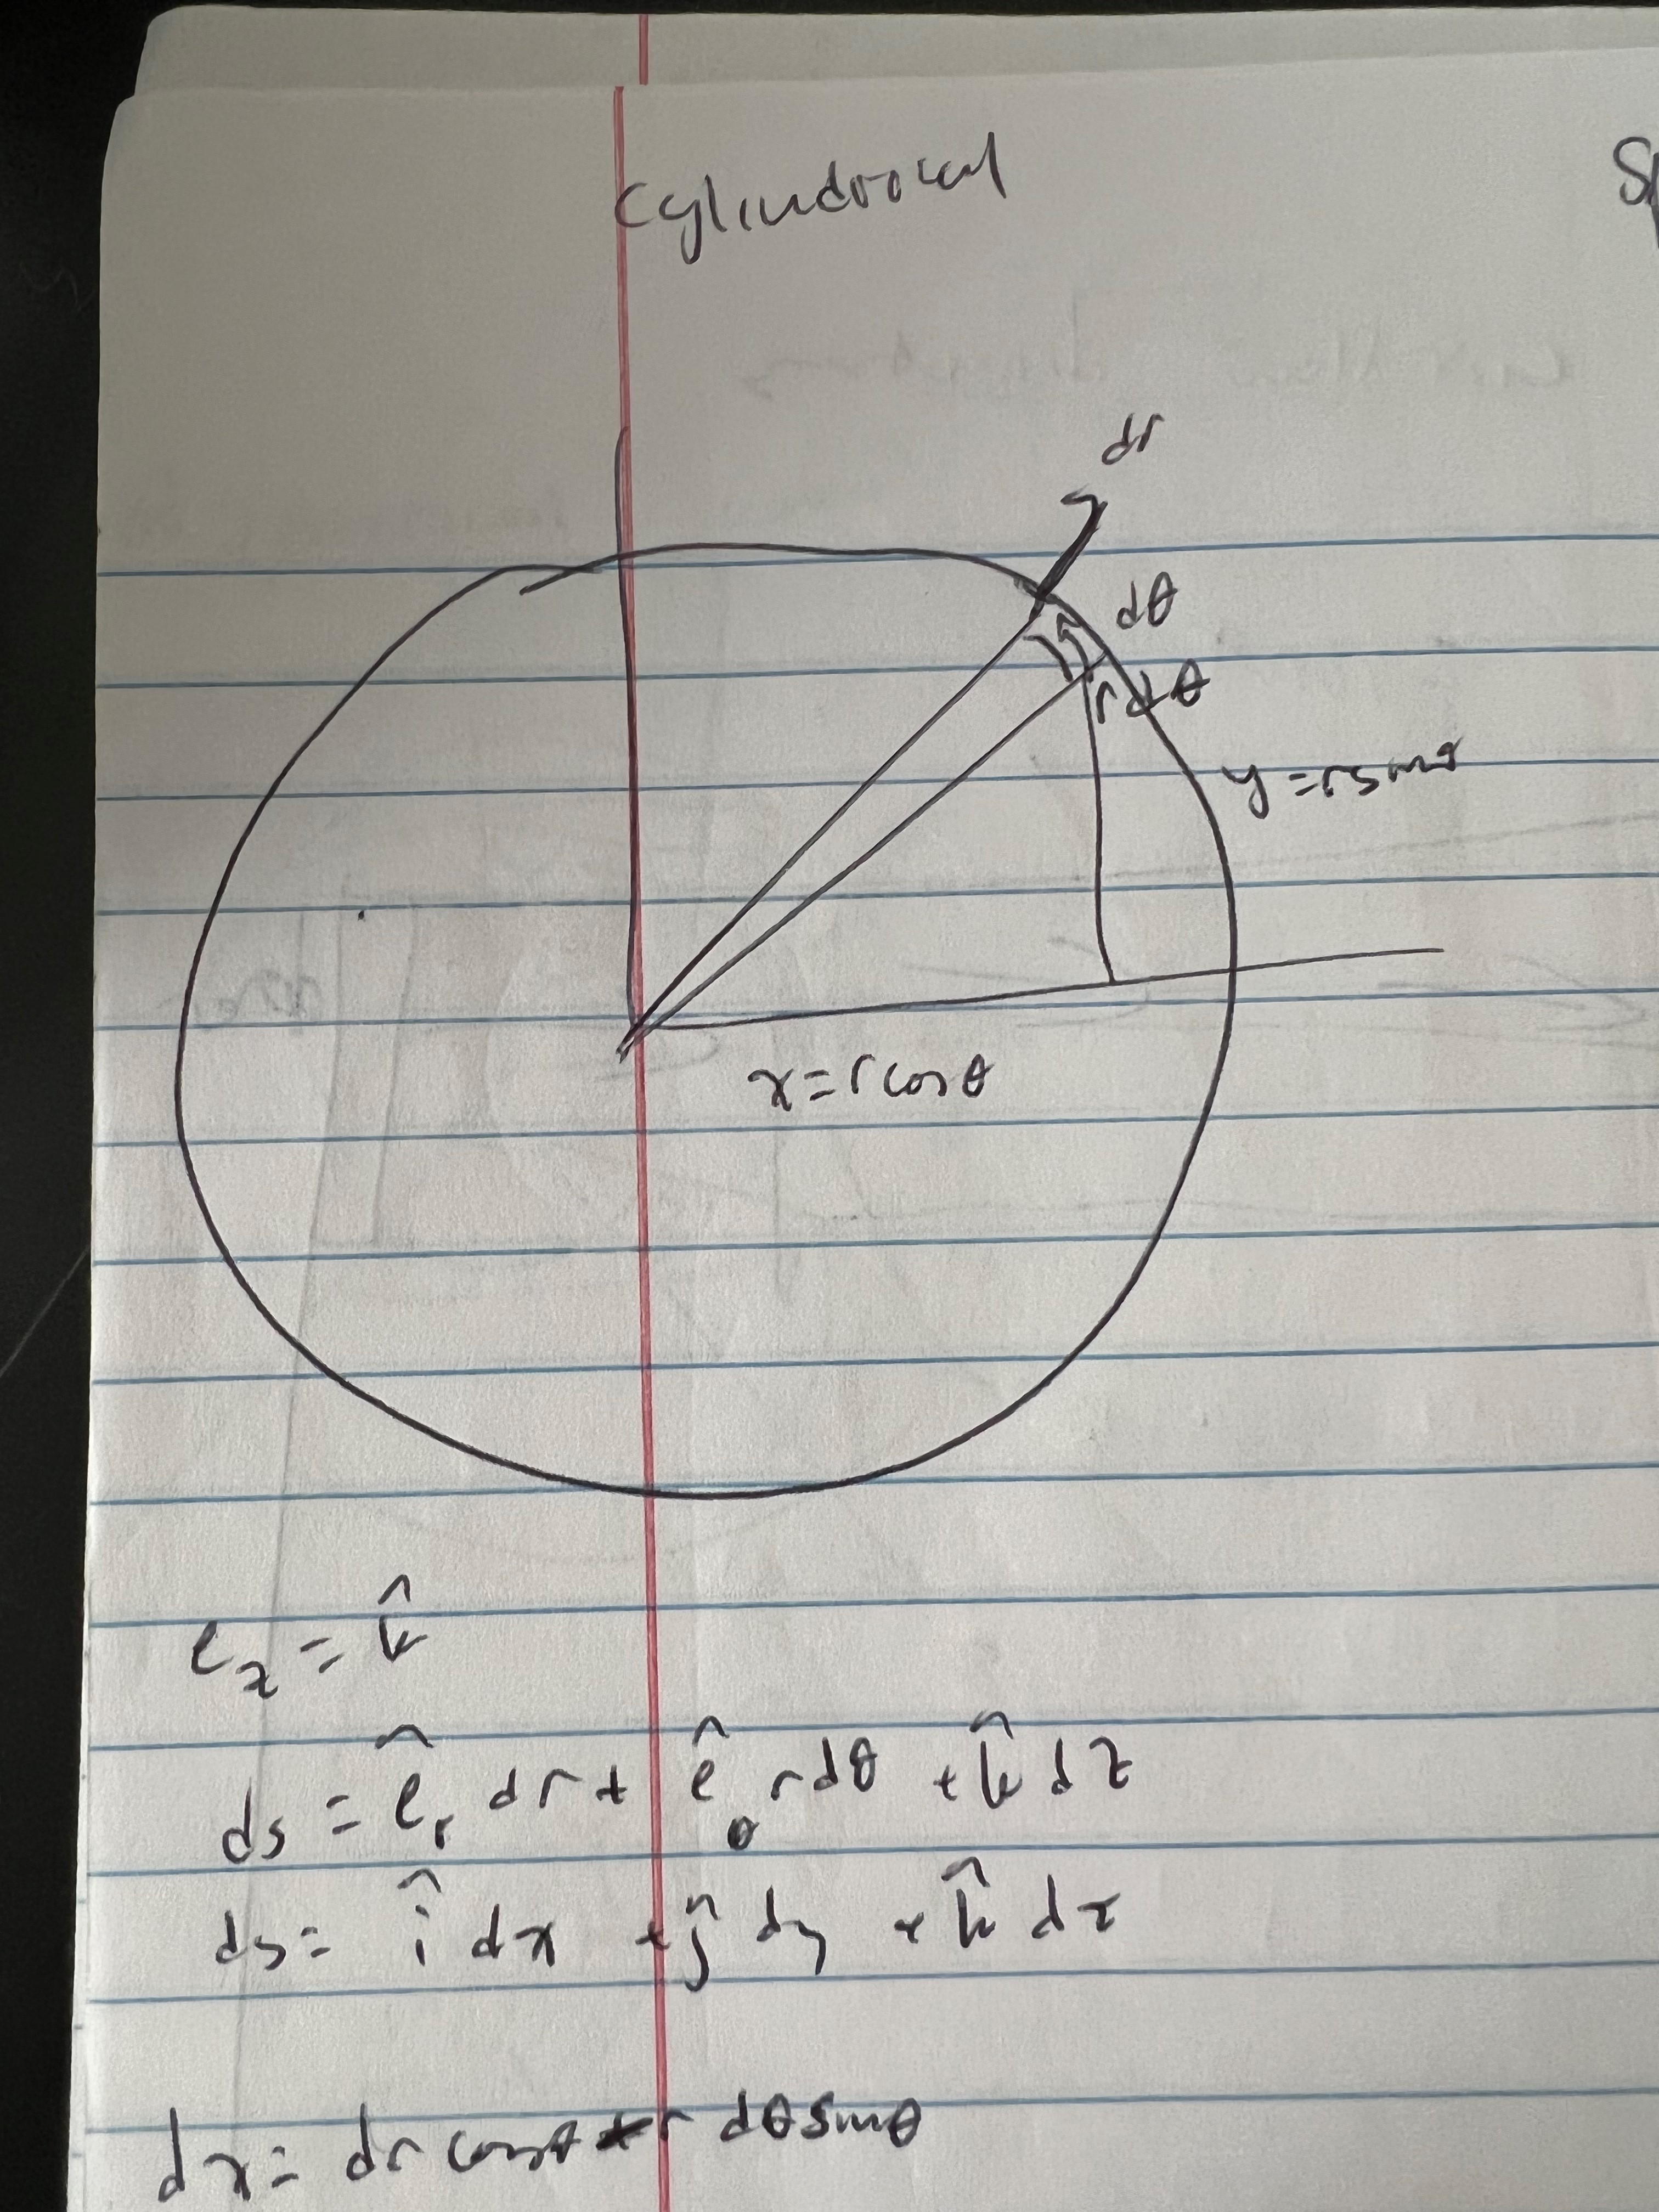
\includegraphics[scale=0.11]{cylindrical.jpg}
        \1 Spherical coordinates: \(\rho,\theta,\phi\)\[dA_\rho=\rho^2\sin\phi d\phi d\theta\qquad dA_\theta=\rho d\rho d\phi\qquad dA_\phi=\rho\sin\phi d\rho d\theta\]\[dV=\rho^2\sin\phi d\phi d\theta d\rho \]
        \1 Visualized: \\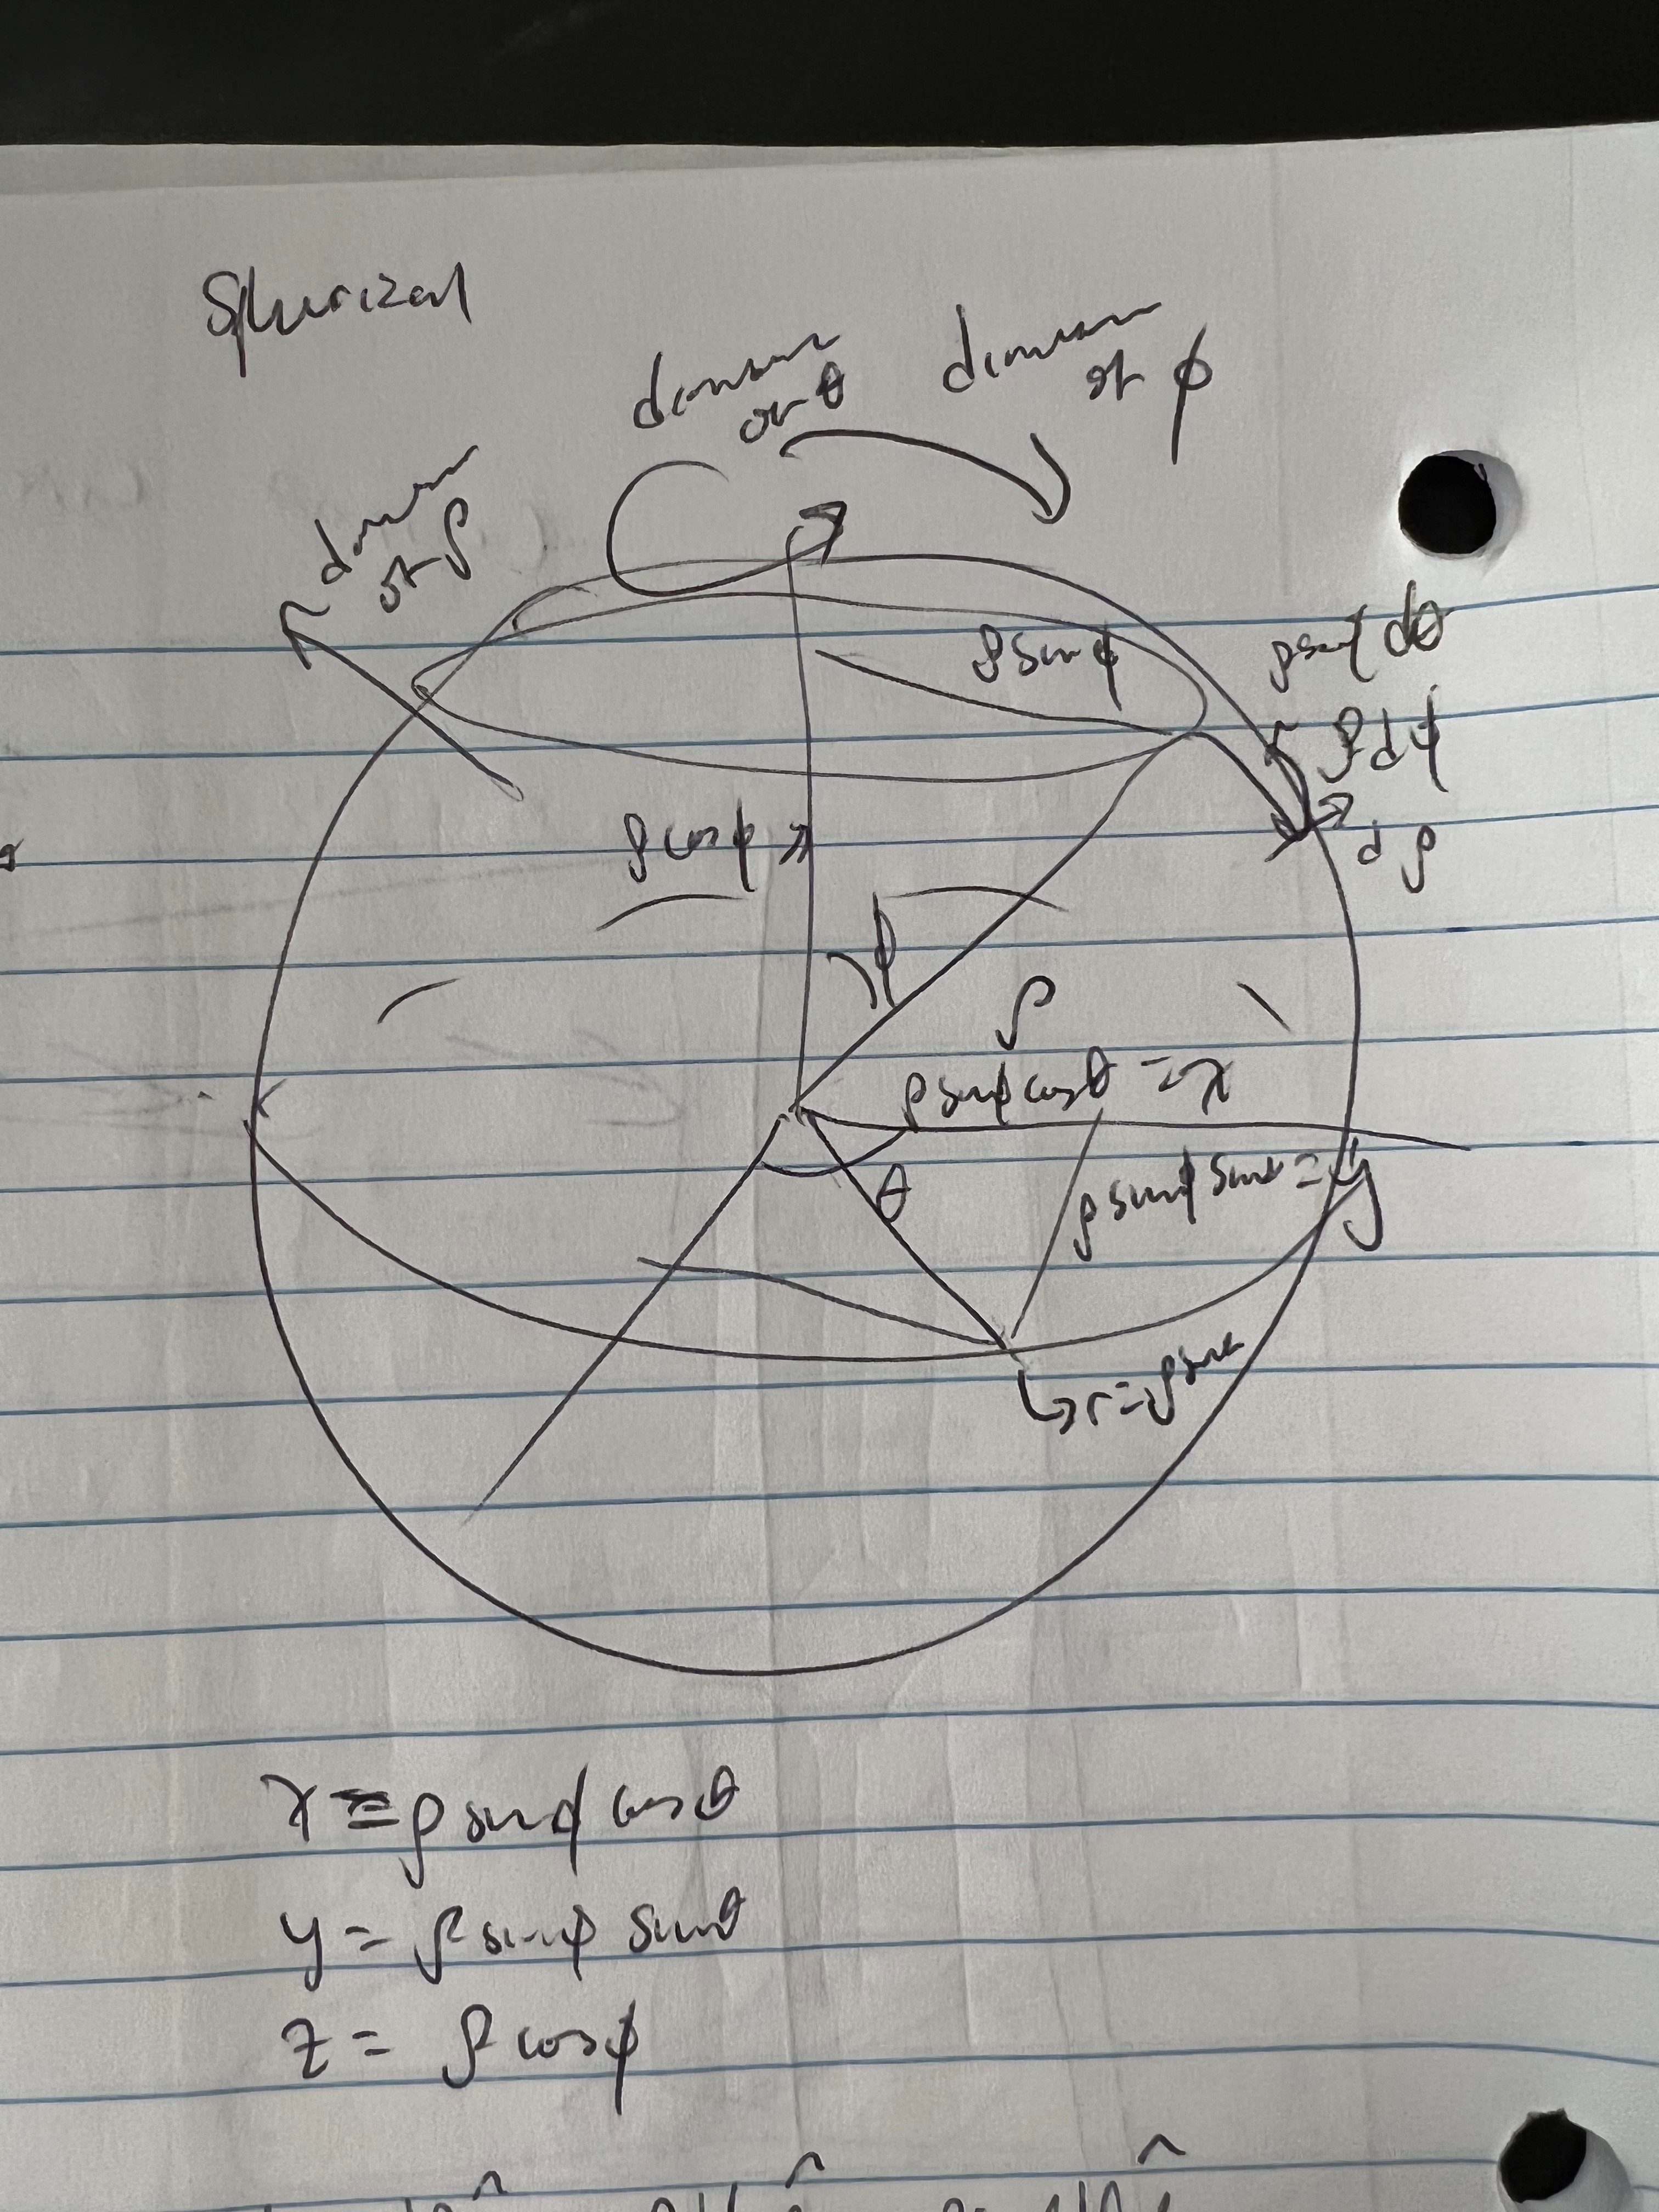
\includegraphics[scale=0.11]{spherical.jpg}

    \end{outline}
\end{document}